%%%%%%%%%%%%%%%%%%%%%%%%%%%%%%%%%%%%%%%%%%%%%%%%%%%%%%%%%%%%%%%%%%%%%%%%%%%%%%%%%%%%%%%%%%%%%%%%%%%%%%%%%%%%%%%%%%%%%%%%%%%%%%%%%%%%%%%%%%%%%%%%%%%%%%%%%%%
% This is just an example/guide for you to refer to when submitting manuscripts to Frontiers, it is not mandatory to use Frontiers .cls files nor frontiers.tex  %
% This will only generate the Manuscript, the final article will be typeset by Frontiers after acceptance.   
%                                              %
%                                                                                                                                                         %
% When submitting your files, remember to upload this *tex file, the pdf generated with it, the *bib file (if bibliography is not within the *tex) and all the figures.
%%%%%%%%%%%%%%%%%%%%%%%%%%%%%%%%%%%%%%%%%%%%%%%%%%%%%%%%%%%%%%%%%%%%%%%%%%%%%%%%%%%%%%%%%%%%%%%%%%%%%%%%%%%%%%%%%%%%%%%%%%%%%%%%%%%%%%%%%%%%%%%%%%%%%%%%%%%

%%% Version 3.4 Generated 2022/06/14 %%%
%%% You will need to have the following packages installed: datetime, fmtcount, etoolbox, fcprefix, which are normally inlcuded in WinEdt. %%%
%%% In http://www.ctan.org/ you can find the packages and how to install them, if necessary. %%%
%%%  NB logo1.jpg is required in the path in order to correctly compile front page header %%%

\documentclass[utf8]{FrontiersinHarvard} % for articles in journals using the Harvard Referencing Style (Author-Date), for Frontiers Reference Styles by Journal: https://zendesk.frontiersin.org/hc/en-us/articles/360017860337-Frontiers-Reference-Styles-by-Journal
%\documentclass[utf8]{FrontiersinVancouver} % for articles in journals using the Vancouver Reference Style (Numbered), for Frontiers Reference Styles by Journal: https://zendesk.frontiersin.org/hc/en-us/articles/360017860337-Frontiers-Reference-Styles-by-Journal
%\documentclass[utf8]{frontiersinFPHY_FAMS} % Vancouver Reference Style (Numbered) for articles in the journals "Frontiers in Physics" and "Frontiers in Applied Mathematics and Statistics" 

%\setcitestyle{square} % for articles in the journals "Frontiers in Physics" and "Frontiers in Applied Mathematics and Statistics" 
\usepackage{url,hyperref,lineno,microtype,subcaption}
\usepackage[onehalfspacing]{setspace}
\usepackage[usenames]{xcolor}
% Tol (2012) colour-blind-, print-, screen-friendly colours, alternative scheme; Munsell terminology
\definecolor{bluepurple}{RGB}{68,119,170}
\definecolor{blue}{RGB}{102,204,238}
\definecolor{green}{RGB}{34,136,51}
\definecolor{yellow}{RGB}{204,187,68}
\definecolor{red}{RGB}{238,102,119}
\definecolor{redpurple}{RGB}{170,51,119}
\definecolor{grey}{RGB}{187,187,187}
\definecolor{lgrey}{RGB}{221,221,221}

\definecolor{notecolour}{RGB}{68,170,153}
%\newcommand*{\puzzle}{\maltese}
\newcommand*{\puzzle}{{\fontencoding{U}\fontfamily{fontawesometwo}\selectfont\symbol{225}}}
\newcommand*{\wrench}{{\fontencoding{U}\fontfamily{fontawesomethree}\selectfont\symbol{114}}}
\newcommand*{\pencil}{{\fontencoding{U}\fontfamily{fontawesometwo}\selectfont\symbol{210}}}
\newcommand{\mynotew}[1]{{\color{notecolour}\wrench\ #1}}
\newcommand{\mynotep}[1]{{\color{notecolour}\pencil\ #1}}
\newcommand{\mynotez}[1]{{\color{notecolour}\puzzle\ #1}}

\usepackage{wrapfig}



\providecommand{\href}[2]{#2}
\providecommand{\eprint}[2]{\texttt{\href{#1}{#2}}}
\newcommand*{\amp}{\&}
% \newcommand*{\citein}[2][]{\textnormal{\textcite[#1]{#2}}%\addtocategory{extras}{#2}
% }
\newcommand*{\citein}[2][]{\textnormal{\cite[#1]{#2}}%\addtocategory{extras}{#2}
}
\newcommand*{\citebi}[2][]{\cite[#1]{#2}%\addtocategory{extras}{#2}
}
\newcommand*{\subtitleproc}[1]{}
\newcommand*{\chapb}{ch.}
%
%\def\UrlOrds{\do\*\do\-\do\~\do\'\do\"\do\-}%
\def\myUrlOrds{\do\0\do\1\do\2\do\3\do\4\do\5\do\6\do\7\do\8\do\9\do\a\do\b\do\c\do\d\do\e\do\f\do\g\do\h\do\i\do\j\do\k\do\l\do\m\do\n\do\o\do\p\do\q\do\r\do\s\do\t\do\u\do\v\do\w\do\x\do\y\do\z\do\A\do\B\do\C\do\D\do\E\do\F\do\G\do\H\do\I\do\J\do\K\do\L\do\M\do\N\do\O\do\P\do\Q\do\R\do\S\do\T\do\U\do\V\do\W\do\X\do\Y\do\Z}%
\makeatletter
%\g@addto@macro\UrlSpecials{\do={\newline}}
\g@addto@macro{\UrlBreaks}{\myUrlOrds}
\makeatother
\newcommand*{\arxiveprint}[1]{%
arXiv \doi{10.48550/arXiv.#1}%
}
\newcommand*{\mparceprint}[1]{%
\href{http://www.ma.utexas.edu/mp_arc-bin/mpa?yn=#1}{mp\_arc:\allowbreak\nolinkurl{#1}}%
}
\newcommand*{\haleprint}[1]{%
\href{https://hal.archives-ouvertes.fr/#1}{\textsc{hal}:\allowbreak\nolinkurl{#1}}%
}
\newcommand*{\philscieprint}[1]{%
\href{http://philsci-archive.pitt.edu/archive/#1}{PhilSci:\allowbreak\nolinkurl{#1}}%
}
\newcommand*{\doi}[1]{%
\href{https://doi.org/#1}{\textsc{doi}:\allowbreak\nolinkurl{#1}}%
}
\newcommand*{\biorxiveprint}[1]{%
bioRxiv \doi{10.1101/#1}%
}
\newcommand*{\osfeprint}[1]{%
Open Science Framework \doi{10.31219/osf.io/#1}%
}
%% symbol = for equality statements within probabilities
\newcommand*{\mo}[1][=]{\mathord{\,#1\,}}
%%
\newcommand*{\sect}{\S}% Sect.~
\newcommand*{\sects}{\S\S}% Sect.~
\newcommand*{\chap}{ch.}%
\newcommand*{\chaps}{chs}%
\newcommand*{\bref}{ref.}%
\newcommand*{\brefs}{refs}%
%\newcommand*{\fn}{fn}%
\newcommand*{\eqn}{eq.}%
\newcommand*{\eqns}{eqs}%
\newcommand*{\fig}{fig.}%
\newcommand*{\figs}{figs}%
\newcommand*{\vs}{{vs}}
\newcommand*{\eg}{{e.g.}}
\newcommand*{\etc}{{etc.}}
\newcommand*{\ie}{{i.e.}}
%\newcommand*{\ca}{{c.}}
\newcommand*{\foll}{{ff.}}
%\newcommand*{\viz}{{viz}}
\newcommand*{\cf}{{cf.}}
%\newcommand*{\Cf}{{Cf.}}
%\newcommand*{\vd}{{v.}}
\newcommand*{\etal}{{et al.}}

%\usepackage{fancybox}
\usepackage{framed}


% \newenvironment{description}{}{}
% \usepackage[shortlabels,inline]{enumitem}
% \SetEnumitemKey{para}{itemindent=\parindent,leftmargin=0pt,listparindent=\parindent,parsep=0pt,itemsep=\topsep}
% \setlist{itemsep=0pt,topsep=\parsep}
% \setlist[enumerate,2]{label=(\roman*)}
% \setlist[enumerate]{label=(\alph*),leftmargin=1.5\parindent}
% \setlist[itemize]{leftmargin=1.5\parindent}
% \setlist[description]{leftmargin=1.5\parindent}

\usepackage{bm}

\usepackage{mathtools}

\usepackage[main=british]{babel}\selectlanguage{british}
%\newcommand*{\langnohyph}{\foreignlanguage{nohyphenation}}
\newcommand{\langnohyph}[1]{\begin{hyphenrules}{nohyphenation}#1\end{hyphenrules}}

\usepackage[autostyle=false,autopunct=false,english=british]{csquotes}
\setquotestyle{american}
\newcommand*{\defquote}[1]{`\,#1\,'}

\usepackage{upgreek}
%% Macros
\DeclarePairedDelimiter\abs{\lvert}{\rvert}
\DeclarePairedDelimiter\set{\{}{\}} %}
\newcommand*{\p}{\mathrm{p}}%probability
\renewcommand*{\P}{\mathrm{P}}%probability
\newcommand*{\E}{\mathrm{E}}
%% The "\:" space is chosen to correctly separate inner binary and external relationss
\renewcommand*{\|}[1][]{\nonscript\:#1\vert\nonscript\:\mathopen{}}
\newcommand*{\defd}{\coloneqq}
\newcommand*{\defs}{\eqqcolon}
\newcommand*{\Land}{\bigwedge}
\newcommand*{\zerob}[1]{\makebox[0pt][c]{#1}}
\newcommand*{\delt}{\updelta}
\newcommand*{\eU}{\bar{U}}
% 
\newcommand*{\ad}{Alzheimer's Disease}
\newcommand*{\mci}{Mild Cognitive Impairment}
\newcommand*{\tjm}{Turing-Jaynes machine}
\newcommand*{\AD}{\mathrm{AD}}
\newcommand*{\nAD}{\lnot\mathrm{AD}}


% Leave a blank line between paragraphs instead of using \\

%\linenumbers


\def\keyFont{\fontsize{8}{11}\helveticabold }
\def\firstAuthorLast{Porta~Mana {et~al.}} %use et al only if is more than 1 author
\def\Authors{P.G.L. Porta~Mana\,$^{1,2,*}$, I.~Rye\,$^{3}$, A.~Vik\,$^{1,2}$, M.~Koci\'nski\,$^{2,4}$, A.~Lundervold\,$^{2,4}$, A.~J.~Lundervold\,$^{3}$, A.~S.~Lundervold\,$^{1,2}$}
% Affiliations should be keyed to the author's name with superscript numbers and be listed as follows: Laboratory, Institute, Department, Organization, City, State abbreviation (USA, Canada, Australia), and Country (without detailed address information such as city zip codes or street names).
% If one of the authors has a change of address, list the new address below the correspondence details using a superscript symbol and use the same symbol to indicate the author in the author list.
\def\Address{$^{1}$Department of Computer Science, Electrical Engineering and Mathematical Sciences, Western Norway University of Applied Sciences, Bergen, Norway \\
$^{2}$Mohn Medical Imaging and Visualization Centre (MMIV), Department of Radiology, Haukeland University Hospital, Bergen, Norway\\
$^{3}$Department of Biological and Medical Psychology, University of Bergen, Norway\\
$^{4}$Department of Biomedicine, University of Bergen, Norway}
% The Corresponding Author should be marked with an asterisk
% Provide the exact contact address (this time including street name and city zip code) and email of the corresponding author
\def\corrAuthor{P.G.L Porta~Mana, HVL, Inndalsveien 28, 5063 Bergen}
\def\corrEmail{pgl@portamana.org}



\setcounter{section}{-1}
\begin{document}
\onecolumn
\firstpage{1}

%\title[Conversion from MCI to AD]{Conversion from MCI to Alzheimer's disease: model-free predictions with quantified uncertainty} 
%\title[Conversion from MCI to AD]{Model-free predictions with quantified uncertainty in personalized medicine: A case study on the conversion from MCI to AD} 
\title[Personalized prognosis \amp\ treatment using a \tjm]{Personalized prognosis \& treatment\\ using Turing-Jaynes machines:\\ An example study on  conversion from Mild Cognitive Impairment to Alzheimer's Disease} 

\author[\firstAuthorLast ]{\Authors} %This field will be automatically populated
\address{} %This field will be automatically populated
\correspondance{} %This field will be automatically populated

\extraAuth{}% If there are more than 1 corresponding author, comment this line and uncomment the next one.
%\extraAuth{corresponding Author2 \\ Laboratory X2, Institute X2, Department X2, Organization X2, Street X2, City X2 , State XX2 (only USA, Canada and Australia), Zip Code2, X2 Country X2, email2@uni2.edu}


\maketitle


\begin{abstract}

%%% Leave the Abstract empty if your article does not require one, please see the Summary Table for full details.
\section{}
\mynotew{TO BE REWRITTEN}

Patients with Mild Cognitive Impairment have an increased risk of a trajectory toward Alzheimer's Disease. Early identification of patients with a high risk of Alzheimer's Disease is essential to provide treatment before the disease is well-established in the brain. great importance to study how well different kinds of predictors
%-- from neuropsychological examinations to advanced brain-imaging techniques -- 
allow us to prognose a trajectory from Mild Cognitive Impairment towards Alzheimer's Disease in an individual patient.

But more is needed for a personalized approach to prognosis, prevention, and treatment, than just the obvious requirement that prognoses be as best as they can be for each patient. Several situational elements that can be different from patient to patient must be accounted for:
\begin{itemize}
\item the \emph{kinds} of clinical data and evidence available for prognosis;
\item the \emph{outcomes} of the same kind of clinical data and evidence;
\item the kinds of treatment or prevention strategies available, owing to different additional medical factors such as physical disabilities, different attitudes toward life, different family networks and possibilities of familial support, different economic means;
\item the advantages and disadvantages, benefits and costs of the same kinds of treatment or prevention strategies; the patient has a major role in the quantification of such benefits and costs;
\item finally, the initial evaluation by the clinician -- which often relies on too subtle clues (family history, regional history, previous case experience) to be considered as measurable data.
\end{itemize}
Statistical decision theory is the normative quantification framework that takes into account these fundamental differences. Medicine has the distinction of having been one of the first fields to adopt this framework, exemplified in brilliant old and new textbooks on clinical decision-making.

Clinical decision-making makes allowance for these differences among patients through two requirements. First, the quantification of prognostic evidence on one side, and of benefits and costs of treatments and prevention strategies on the other, must be clearly separated and handled in a modular way. Two patients can have the same prognostic evidence and yet very different prevention options. Second, the quantification of independent prognostic evidence ought to be in the form of \emph{likelihoods about the health condition} (or equivalently of likelihood ratios, in a binary case), that is, of the probabilities of the observed test outcomes given the hypothesized health conditions. Likelihoods from independent clinical tests and predictors can then be combined with a simple multiplication; for one patient, we could have three kinds of predictor available; for another, we could have five. The clinician's pre-test assessment is included in the form of a probability. These patient-dependent probabilities are combined with the patient-dependent costs and benefits of treatment or prevention to arrive at the best course of action for that patient. The main result underlying statistical decision theory is that decision-making \emph{must} take this particular mathematical form in order to be optimal and logically consistent.

The present work investigates the prognostic power of a set of neuropsychological and Magnetic Resonance Imaging examinations, demographic data, and genetic information about Apolipoprotein-E4The present work investigates the prognostic power of a set of neuropsychological and Magnetic Resonance Imaging examinations, demographic data, and genetic information about Apolipoprotein-E4 (APOE) status, for the prediction of the onset of Alzheimer's Disease in patients defined as mildly cognitively impaired at a baseline examination. The longitudinal data used come from the ADNI database.

 (APOE) status, for the prediction of the onset of Alzheimer's disease in patients defined as mildly cognitively impaired at a baseline examination. The longitudinal data used come from the ADNI database.

The prognostic power of these predictors is quantified in the form of a combined likelihood for the onset of Alzheimer's disease. As a hypothetical example application of personalized clinical decision making, three patient cases are considered where a clinician starts with prognostic uncertainties, possibly coming from other tests, of 50\%/50\%, 25\%/75\%, 75\%/25\%. It is shown how these pre-test probabilities are changed by the predictors. \mynotew{update this}

\mynotew{rewrite following} This quantification also allows us to rank the relative prognostic power of the predictors. It is found that several neuropsychological examinations have the highest prognostic power, much higher than the genetic and imaging-derived predictors included in the present set.

Several additional advantages of this quantification framework are also exemplified and discussed in the present work:
\begin{itemize}
\item missing data are automatically handled, and results having partial data are not discarded; this quantification, therefore, also accounts for patient-dependent availability of \emph{non-independent} predictors;
\item no modelling assumptions (e.g.,\ linearity, gaussianity, functional dependence) are made;
\item the prognostic power obtained is intrinsic to the predictors, that is, it is a bound for \emph{any} prognostic algorithm;
\item variability ranges of the results owing to the finite size of the sample data are automatically quantified.
\item the values obtained, being probabilities, are more easily interpretable than scores of various kinds.
\end{itemize}


%Alzheimer's disease (AD) is by far the most common type of dementia. The disease is characterized by an insidious onset caused by neurodegenerative processes, which lead to progressive loss of cognitive and functional abilities. Alongside the devastating personal consequences AD has on those affected and their caregivers, economical costs related to the disease are massive.
% 
% One of the difficulties for successful treatment of AD is the fact that its pathological hallmarks tend to be established in the brain decades prior to the time a person's cognitive and functional impairments are severe enough to get medical attention. Management of known risk factors for AD (e.g., high blood pressure and diabetes) is therefore emphasized. Recent studies point towards promising life-style interventions reducing AD-pathology and neurodegeneration and delaying symptom-onset. Much effort is therefore put into early identification and treatment of patients in the prodromal phase of the disease. Mild Cognitive Impairment (MCI) has become a diagnostic concept to describe this phase. Individuals falling within this diagnostic category show a cognitive decline greater than expected in normal cognitive aging, but still not with the severity of functional impairment characterizing those with dementia.


% \color{yellow}{\tiny For full guidelines regarding your manuscript please refer to \href{http://www.frontiersin.org/about/AuthorGuidelines}{Author Guidelines}.

% As a primary goal, the abstract should render the general significance and conceptual advance of the work clearly accessible to a broad readership. References should not be cited in the abstract. Leave the Abstract empty if your article does not require one, please see \href{http://www.frontiersin.org/about/AuthorGuidelines#SummaryTable}{Summary Table} for details according to article type.

% } 


\tiny
 \keyFont{\section{Keywords:} Clinical decision making, Utility theory, Probability theory, Artificial Intelligence, Machine Learning, Base-rate fallacy} %All article types: you may provide up to 8 keywords; at least 5 are mandatory.
\end{abstract}

\section{Each patient is unique}

%%%% EXAMPLE-PATIENT DATA %%%%
% Olivia, Ariel, Bianca:
% Apoe4_             0.00000000
% ANARTERR_neuro    18.00000000
% AVDEL30MIN_neuro   5.00000000 Ravlt-del
% AVDELTOT_neuro    10.00000000 Ravlt-rec
% CATANIMSC_neuro   21.00000000
% GDTOTAL_gds        3.00000000
% RAVLT_immediate   36.00000000
% TRAASCOR_neuro    21.00000000
% TRABSCOR_neuro   114.00000000
% AGE               75.38823609
% LRHHC_n_long       0.00425972
% Gender_num_        1.00000000
%
% posterior Olivia, Bianca:  0.301679
% prior Ariel: 0.65
% likelihood Ariel cAD:  8.97179e-12
% likelihood Ariel sMCI:  1.85685e-11
% posterior Ariel: 0.47294
%%%%%%%%%
% Curtis:
% Apoe4_             1.00000000
% ANARTERR_neuro    15.00000000
% AVDEL30MIN_neuro   0.00000000
% AVDELTOT_neuro     3.00000000
% CATANIMSC_neuro   14.00000000
% GDTOTAL_gds        2.00000000
% RAVLT_immediate   20.00000000
% TRAASCOR_neuro    36.00000000
% TRABSCOR_neuro   126.00000000
% AGE               63.82721344
% LRHHC_n_long       NA
% Gender_num_        0.00000000
%
% posterior 0.70256
%
%%%%%%%%
% Utility matrix Olivia, Ariel, Curtis:
% #1  1.0  0.0
% #2  0.9  0.3
% #3  0.8  0.5
% #4  0.0  1.0
%%%%
% Utility matrix Bianca:
% #1  1.0  0.0
% #2  0.8  0.3
% #3  0.7  0.5
% #4  0.0  1.0
%%%%%%%%
% optimal treatments
% Olivia #2
% Ariel #3
% Bianca #1
% Curtis #4

Meet Olivia, Ariel, Bianca, Curtis.\footnote{Fictive characters; any reference to real persons is purely coincidental}
% names from Shakespeare's plays
These four persons don't know each other, but they have something in common: they all suffer from a mild form of cognitive impairment, and are afraid that their impairment will turn into Alzheimer's Disease within a couple of years. In fact, this is why they recently underwent some clinical analyses and cognitive tests. Today they received the results of their analyses. From these results, available clinical statistical data, and other relevant information, their clinician will assess their risk of developing Alzheimer. The clinician and each patient will then decide among a set of possible preventive treatments.

Besides this shared condition and worry, these patients have other things in common -- but also some differences. Let's take Olivia as reference and list the similarities and difference between her and the other three:
\begin{itemize}
\item Olivia and Ariel turn out to have exactly identical clinical results and age. They would also get similar benefits from the available preventive-treatment options. Ariel, however, comes from a different geographical region with a higher rate of conversion, and from a family with a heavy history of Alzheimer's Disease, unlike Olivia. Because of this family background, the clinician judges a priori a 65\% probability that Ariel's cognitive impairment will convert to Alzheimer's Disease

\item Olivia and Bianca also have exactly the same clinical results and age. They come from the same geographical region and have very similar family histories. In fact we shall see that they have the same probability of developing Alzheimer's disease. Bianca, however, suffers from several allergies and additional clinical conditions that render some of the preventive options slightly riskier for her.

\item Olivia and Curtis have different clinical results. In particular, Olivia does not have the risky Apolipoprotein-E4 (APOE4) allele \citep{liuetal2013} whereas Curtis has, and Olivia is more than 10 years older than Curtis. But they otherwise come from the same geographical region, have very similar family histories, and would get similar benefits from the preventive options. Note that one clinical result of Curtis's (hippocampal volume) is missing.
\end{itemize}

We can categorize these differences as \enquote{difference in auxiliary information} (Olivia and Ariel), \enquote{difference in preventive benefits} (Olivia and Bianca), \enquote{difference in clinical predictors} (Olivia and Curtis). Table~\ref{tab:patients_data} reports the clinical results and demographic data common to Olivia, Ariel, Bianca, as well as those of Curtis \mynotew{need to explain the variates and refer to \citep{ryeetal2022}}. The figure on its side summarizes the similarity and differences between Olivia and the other three patients. 
% \begin{figure}[!h]% with figure
%  \centering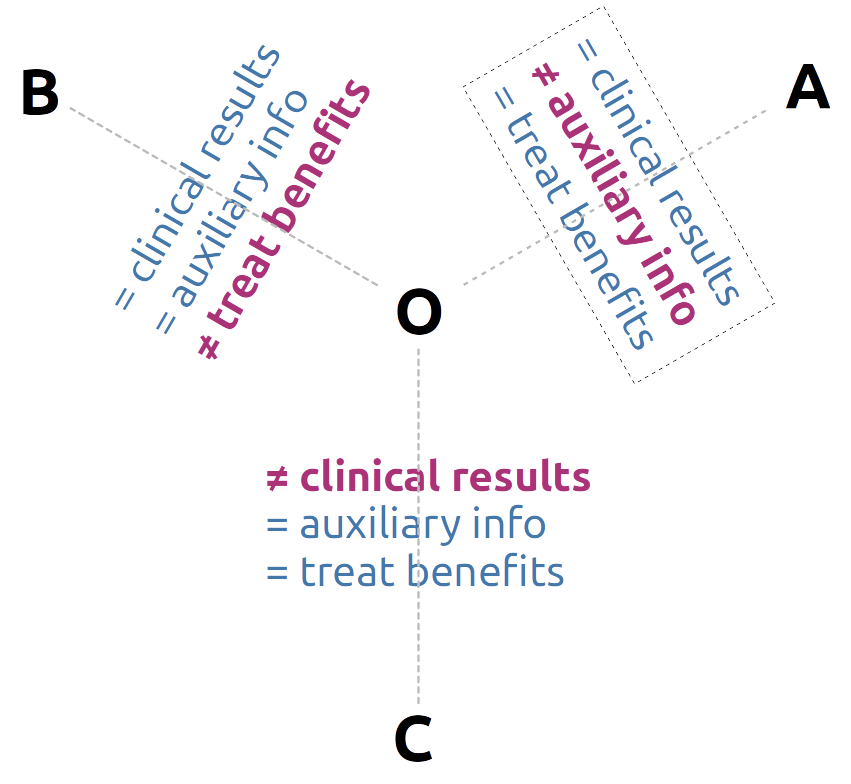
\includegraphics[width=0.25\linewidth]{OABC.png}\\
% \caption{\mynotep{draft, needs better font sizes}}\label{fig:OABC}
% \end{figure}%
\begin{table}[!h]
  \centering
  \begin{tabular}{lcccc}
    \hline\\[-1.5\jot]
    &{\small Olivia} &{\small Ariel} &{\small Bianca} &{\small Curtis}
    \\[\jot]
    Age&75.4&75.4&75.4&63.8 \\
    Sex&F&F&F&M \\
    HC${}/10^{-3}$&4.26&4.26&4.26&[missing] \\
    APOE4&N&N&N&Y \\
    ANART&18&18&18&15 \\
    CFT&21&21&21&14 \\
    GDS&3&3&3&2 \\
    RAVLT-im&36&36&36&20 \\
    RAVLT-del&5&5&5&0 \\
    RAVLT-rec&10&10&10&3 \\
    TMTA&21&21&21&36 \\
    TMTB&114&114&114&126
    \\[\jot]
    \hline
  \end{tabular}\hspace{2em}
  \begin{minipage}{0.4\linewidth}
    \centering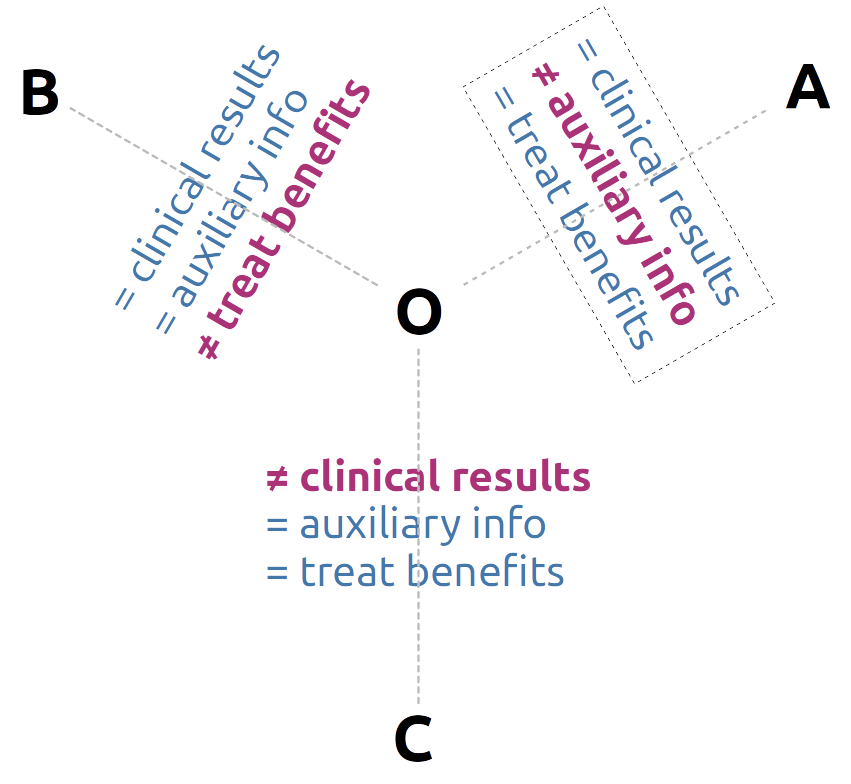
\includegraphics[width=\linewidth]{OABC.png}\\
    % \caption{\mynotep{draft, needs better font sizes}}\label{fig:OABC}
  \end{minipage}
  \caption{\mynotew{Clinical results \& demographic data}}\label{tab:patients_data}
  % \begin{tabular}{ccccccccccccc}
  %   Patient&
  %   Age&Sex&HC${}\cdot 10^{-3}$&APOE4&
  %   ANART&CFT&GDS&RAVLT-im&RAVLT-del&RAVLT-rec&TMTA&TMTB
  %   \\[1\jot]
  %   \emph{Olivia, Ariel, Bianca}&
  %   75.4&F&4.26&N&
  %   18&21&3&36&5&10&21&114
  %   \\
  %   \emph{Curtis}&
  %   63.8&M&[missing]&Y&
  %   15&14&2&20&0&3&36&126
  % \end{tabular}
\end{table}

\medskip

Considering the similarities and differences among these patients, which treatments are optimal and should prescribed to them?

\medskip

Our main purpose in the present work is to illustrate, using the four fictitious patients above as example, how this clinical decision-making problem can today be solved methodically, exactly, and at low computational cost, when the available prognostic clinical information involves one-dimensional or categorical variates such as those listed in table~\ref{tab:patients_data}. The solution method integrates available clinical statistical data with each new patient's unique combination of clinical results, auxiliary information, and treatment benefits. % It is therefore the staple method for personalized prognosis, diagnosis, treatment.

In our example we shall find that -- despite the many factors in common among our four patients, even despite the identical clinical results for Olivia, Ariel, Bianca, and despite the identical probability of conversion for Olivia and Bianca -- \emph{the optimal treatment option for each patient is different from those for the other three}. This result exemplifies the importance of differences among patients with regard to clinical results, auxiliary information, or preventive benefits.

The method used is none other than decision theory, the combination of probability theory and utility theory \citep[\chaps~13--14]{vonneumannetal1944_r1955,raiffaetal1961_r2000,raiffa1968_r1970,lindley1971_r1988,kreps1988,jaynes1994_r2003}. Medicine has the distinction of having been one of the first fields to adopt it \citep{ledleyetal1959}, with old and new brilliant textbooks \citep{weinsteinetal1980,soxetal1988_r2013,huninketal2001_r2014} that explain and exemplify its application.

Decision theory is also the normative foundation for the construction of an Artificial Intelligence agent capable of rational inference and decision making \citetext{\citealp[\chap~IV]{russelletal1995_r2022}; \citealp[\chaps~1--2]{jaynes1994_r2003}}. The present method can therefore be seen as the application of an ideal machine-learning algorithm. We call it the \emph{Turing-Jaynes machine}  in homage to Turing, who put these principles into practice with automated devices \citep{good1979}, and Jaynes, who clearly explained the inductive logic behind such a machine \citep{jaynes1994_r2003}. The \tjm\ is \enquote{ideal} in the sense of being free from approximations, special modelling assumptions, and limitations in its informational output; not in the sense of being impracticable. In the present work we indeed show that for some kinds of dataset such ideal machine-learning algorithm is a reality. It is preferable to popular algorithms such as neural networks, random forests, support-vector machines, which are unsuited to clinical decision-making problems owing to their output limitations. We discuss this matter further in \sect\mynotew{***}.

%%%% Note on "predictand"
%
% The quantity that we want to forecast is in various texts called "dependent variable" or "response variable". I personally don't like either. Both can be misleading. Surely AD-conversion is not "dependent" on cognitive variates, for example. Moreover we'll see that we are actually swapping the role of "independent" and "dependent" variables in this work. Same goes for "response". With a readership of medical scientists it's best to avoid the special connotations of these words, leaving them for variables that are indeed biologically dependent.
%
% This leaves us with "predictand", literally "the thing that has to be predicted", which is exactly what AD-conversion is. I believe this term is used in climate science and meteorology. It's good because it does not misleadingly imply that AD-conversion biologically depends or is a consequence of other variables.
%%%%

\mynotep{Add other advantages of the \tjm: 
  \begin{itemize}
  \item it does not make assumptions, besides natural assumption of smoothness of full-population frequency distribution
  \item can be used with partially missing clinical data
  \item can be used with binary or continuous predictands
  \item it tells us the maximum predictive power of the predictors
  \item it quantifies how prediction could change if we had more sample data
  \item it can be applied on-the-fly to each new patient
  \end{itemize}
  and goals, results, and some synopsis}

The inferential and decision-making steps based on the \tjm\ are summarized in table~\ref{tab:inference_decision_steps}.
\begin{table}[!h]  
  \centering
  \begin{framed}
    \mynotew{To be redone}
    \caption{Inferential and decision-making steps. Steps in \textbf{boldface} represent patient-dependent, personalized steps that cannot be obtained from the learning dataset}\label{tab:inference_decision_steps}

    \vspace{1em}
    
    \begin{enumerate}\itemsep1em 
    \item\label{item:learn} Infer the full-population frequencies of predictors and predictand with the \tjm,  using available datasets.
    \item\label{item:population} \textbf{Assess in respect of which variates the present patient can be considered as belonging to the same population underlying the learning dataset.}
    \item\label{item:prior} \textbf{Assess the prior probability of the predictand for the present patient.} This step allows us (a) to consider additional clinical information outside of the dataset's variates, and available for the present patient only; (b) to correct for mismatches between the dataset's underlying population and the patient's one.
      
    \item\label{item:likelihood}Calculate the \emph{likelihood}
      % -- as opposed to the probability --
      of the predictand for a specific patient, given the patient's predictor values. Combine this likelihood with the prior from step~\ref{item:prior}, to obtain the final probability for the predictand, for the present patient.

    \item\label{item:utilities} \textbf{Assess the clinical courses of action available for the present patient, together their benefits and costs.} This step is fundamentally patient-dependent and is the one open to most variability from patient to patient.

    \item\label{item:expected_utility} Choose the course of action having maximal expected benefit for the present patient, given the benefits assessed in step~\ref{item:utilities} and the final probability assessed in step~\ref{item:likelihood}.  
    \end{enumerate}
  \end{framed}
\end{table}

These steps will be explained and illustrated in the next three sections, presented in chronological order as the clinician would apply them. They could also be presented in reverse order, more suited to their logical dependence, because the procedure in each one is motivated by the next. We suggest that readers familiar with the principles of clinical decision making read them in \sect\,\ref{sec:learning_step}-\sect\,\ref{sec:population_step}-\sect\,\ref{sec:utilities_step} order; whereas readers unfamiliar with these principles (who may include readers with a specialized background in machine learning) read them in \sect\,\ref{sec:utilities_step}-\sect\,\ref{sec:population_step}-\sect\,\ref{sec:learning_step} order.


\section{Learning}
\label{sec:learning_step}

In the learning stage the \tjm\ infers, from a given sample dataset, the statistical relationships of a large population of which our future patients can be considered members, at least in some respects. Such relationships will help us in our prognoses. The basic idea is intuitive. If a patient can be considered a member of some population, and if we knew the joint frequencies of all possible combinations of predictor and predictand values in such population -- and knew nothing else -- then we would say that the probability for the patient to have particular values is equal to the population frequency. Pure symmetry considerations lead to this intuitive result \citep[\sects~4.2--4.3]{definetti1930,dawid2013,bernardoetal1994_r2000}.

But it must be emphasized, and it is essential for our method, that it is \emph{not} necessary (and is seldom true) that a future patient be considered as a member of such a population \emph{in all respects}. A patient can be considered a member only \emph{conditionally} on particular variate values. We shall discuss this point with an example in \sect~\ref{sec:population_step}.

If the full statistics of such a population were known, our task would just be to \enquote{enumerate} rather than to \enquote{learn}. Learning comes into play because the full population is not known: we only have a sample from it.

The \tjm\ assigns a probability to each possible frequency distribution for the full population. It determines the probability of each \enquote{candidate} frequency distribution by combining two factors: (a) how well the candidate fits the sample data, (b) how biologically or physically reasonable the candidate is. Figure~\ref{fig:inferring_distribution} show a fictitious sample data and various candidate frequency distributions \mynotep{...}.
\begin{figure}[!t]% with figure
  \centering%
  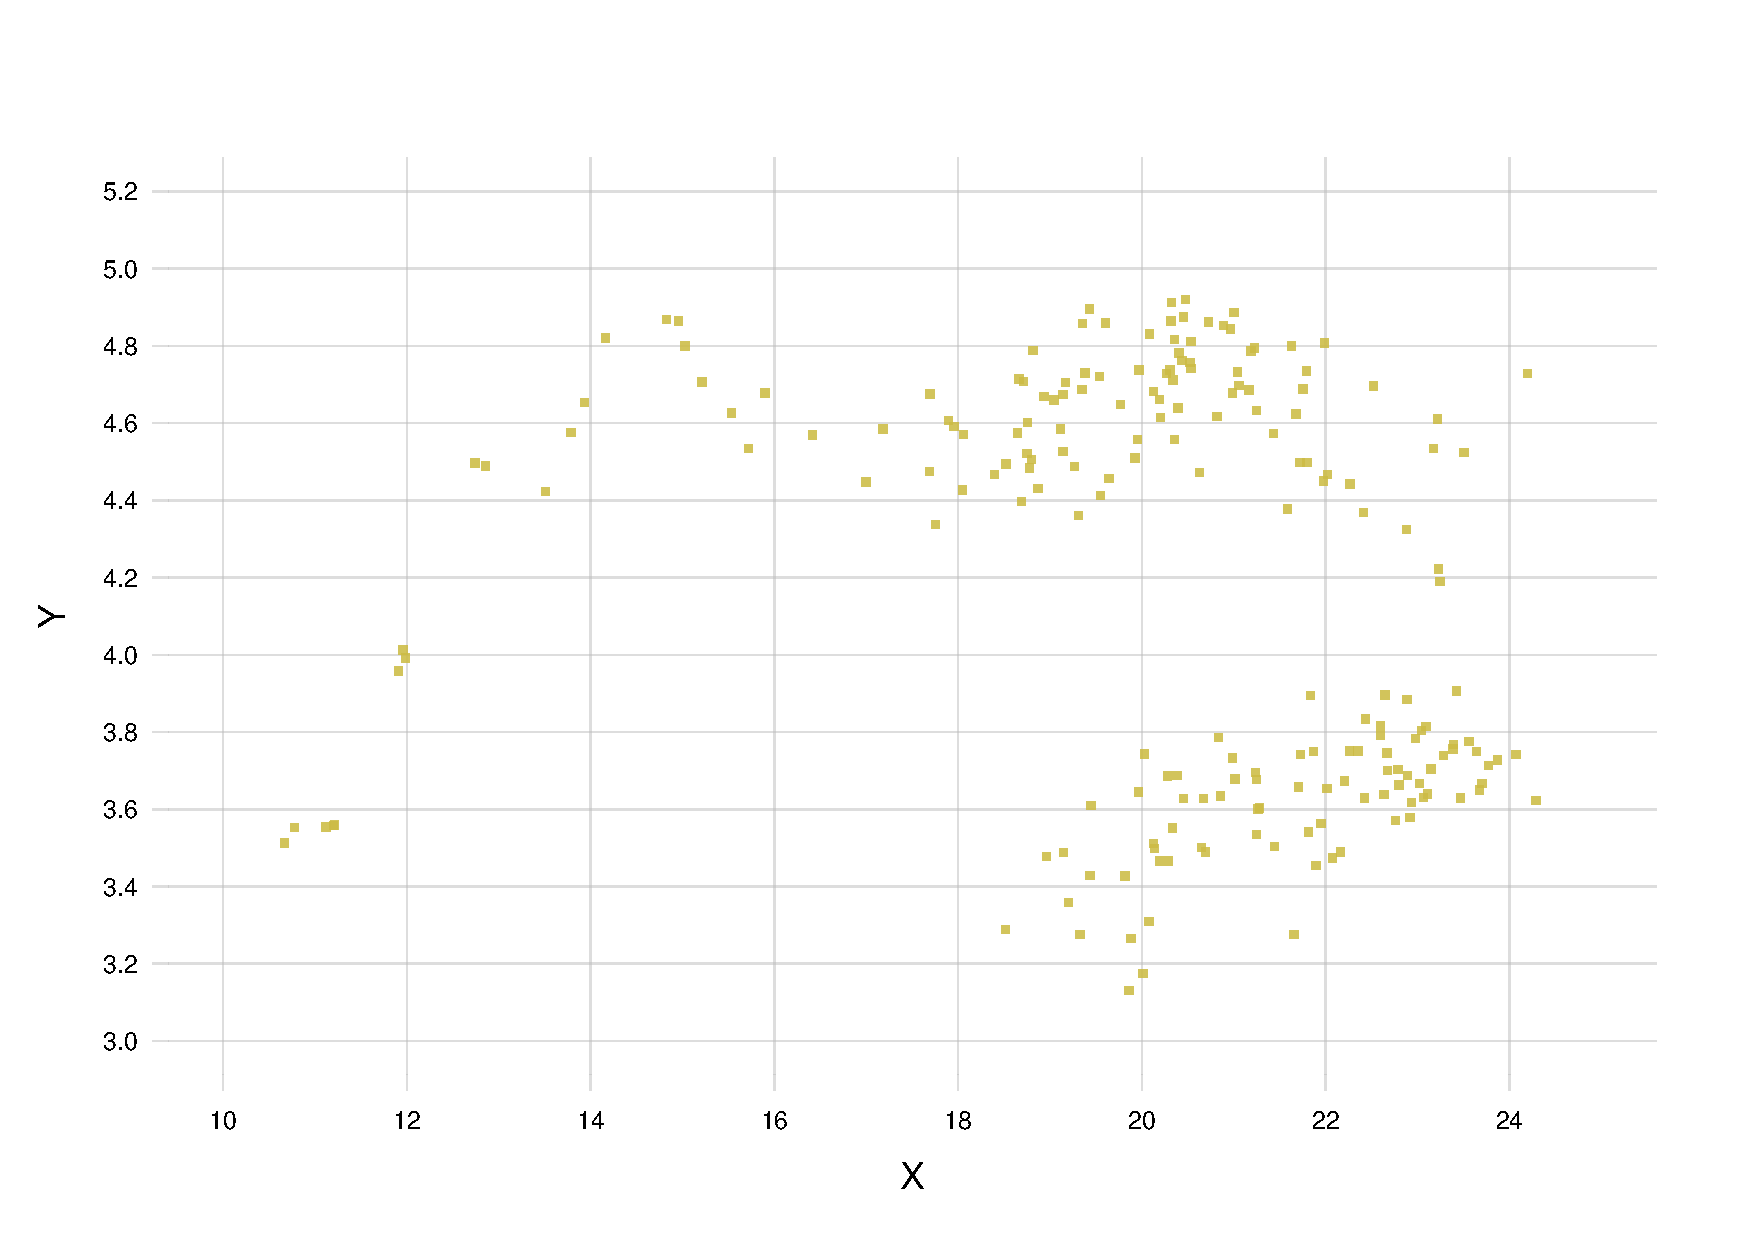
\includegraphics[width=0.49\linewidth]{exampledistr_sample_all.pdf}
  \hfill
  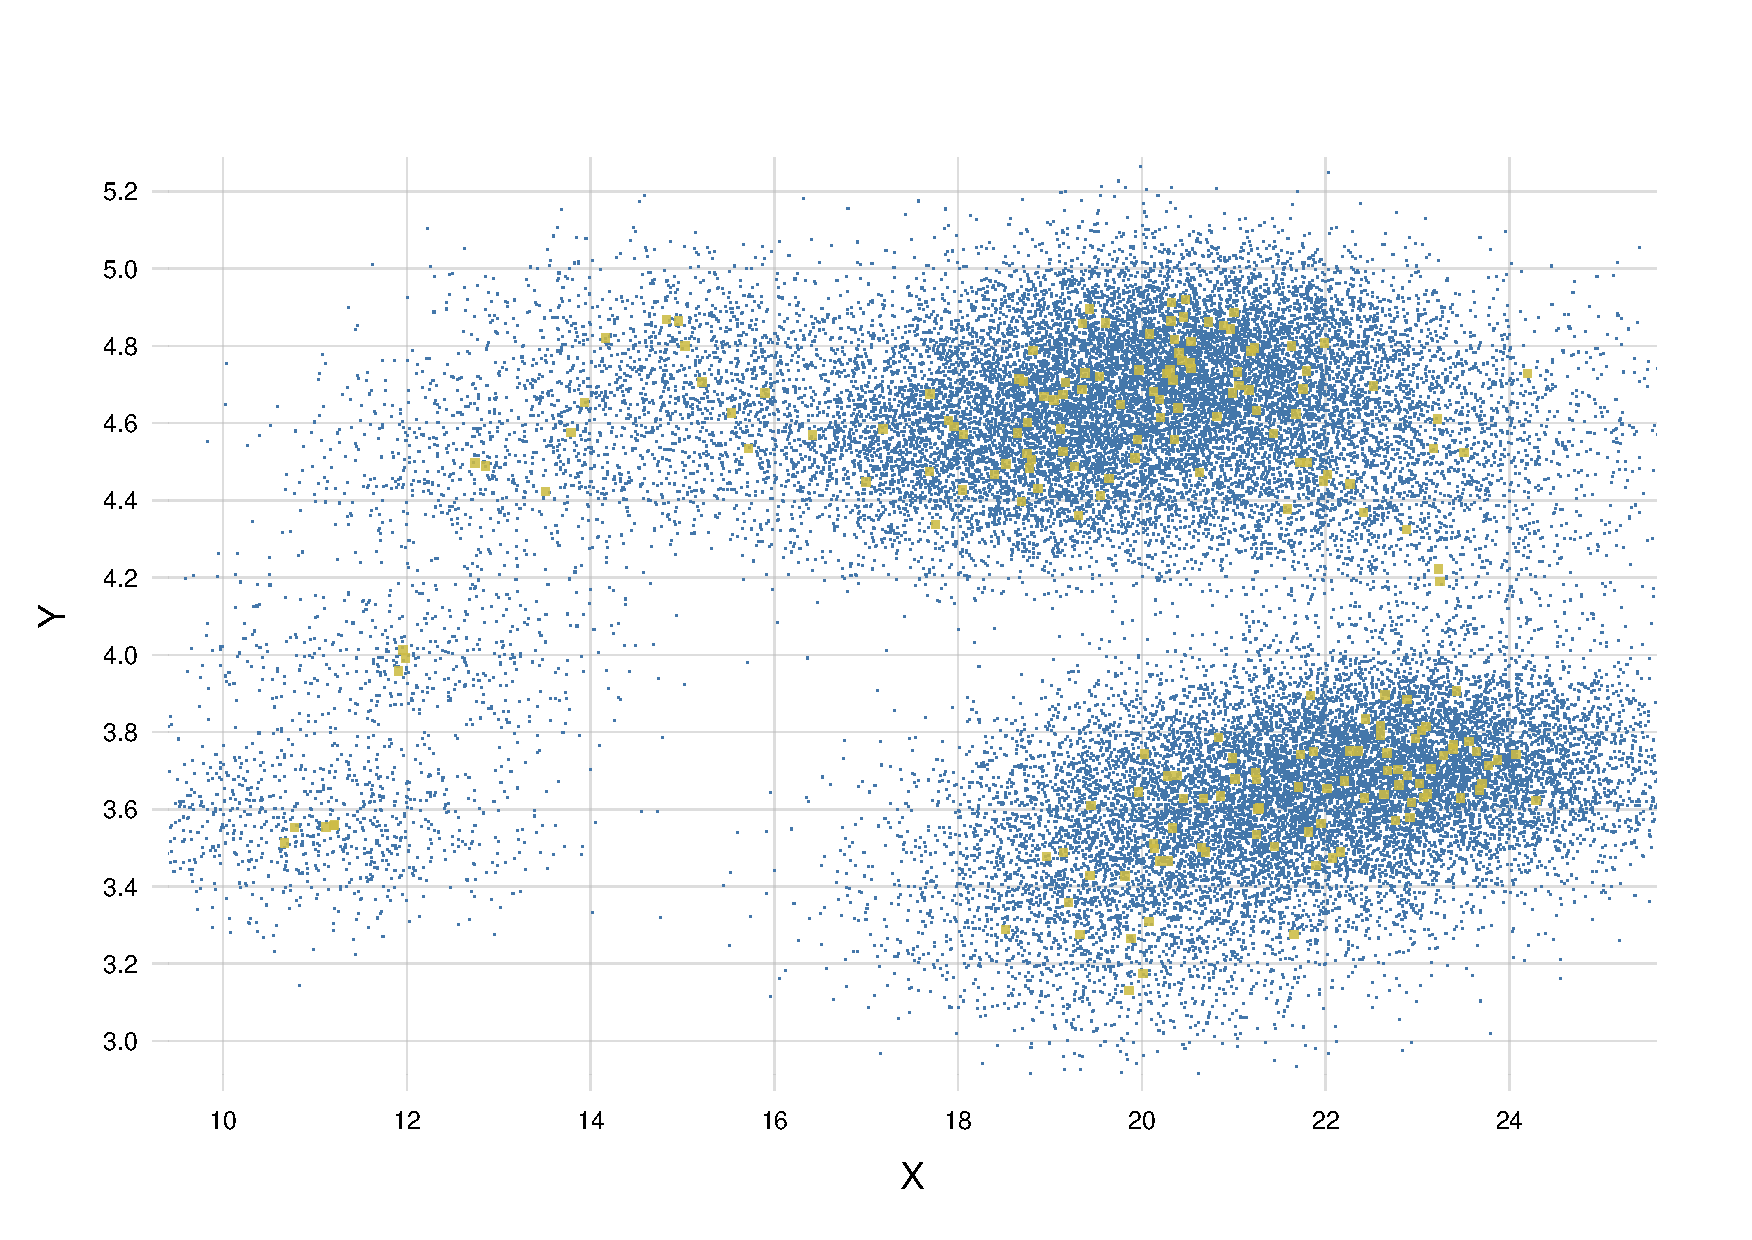
\includegraphics[width=0.49\linewidth]{exampledistr_okish_all.pdf}
  \\
  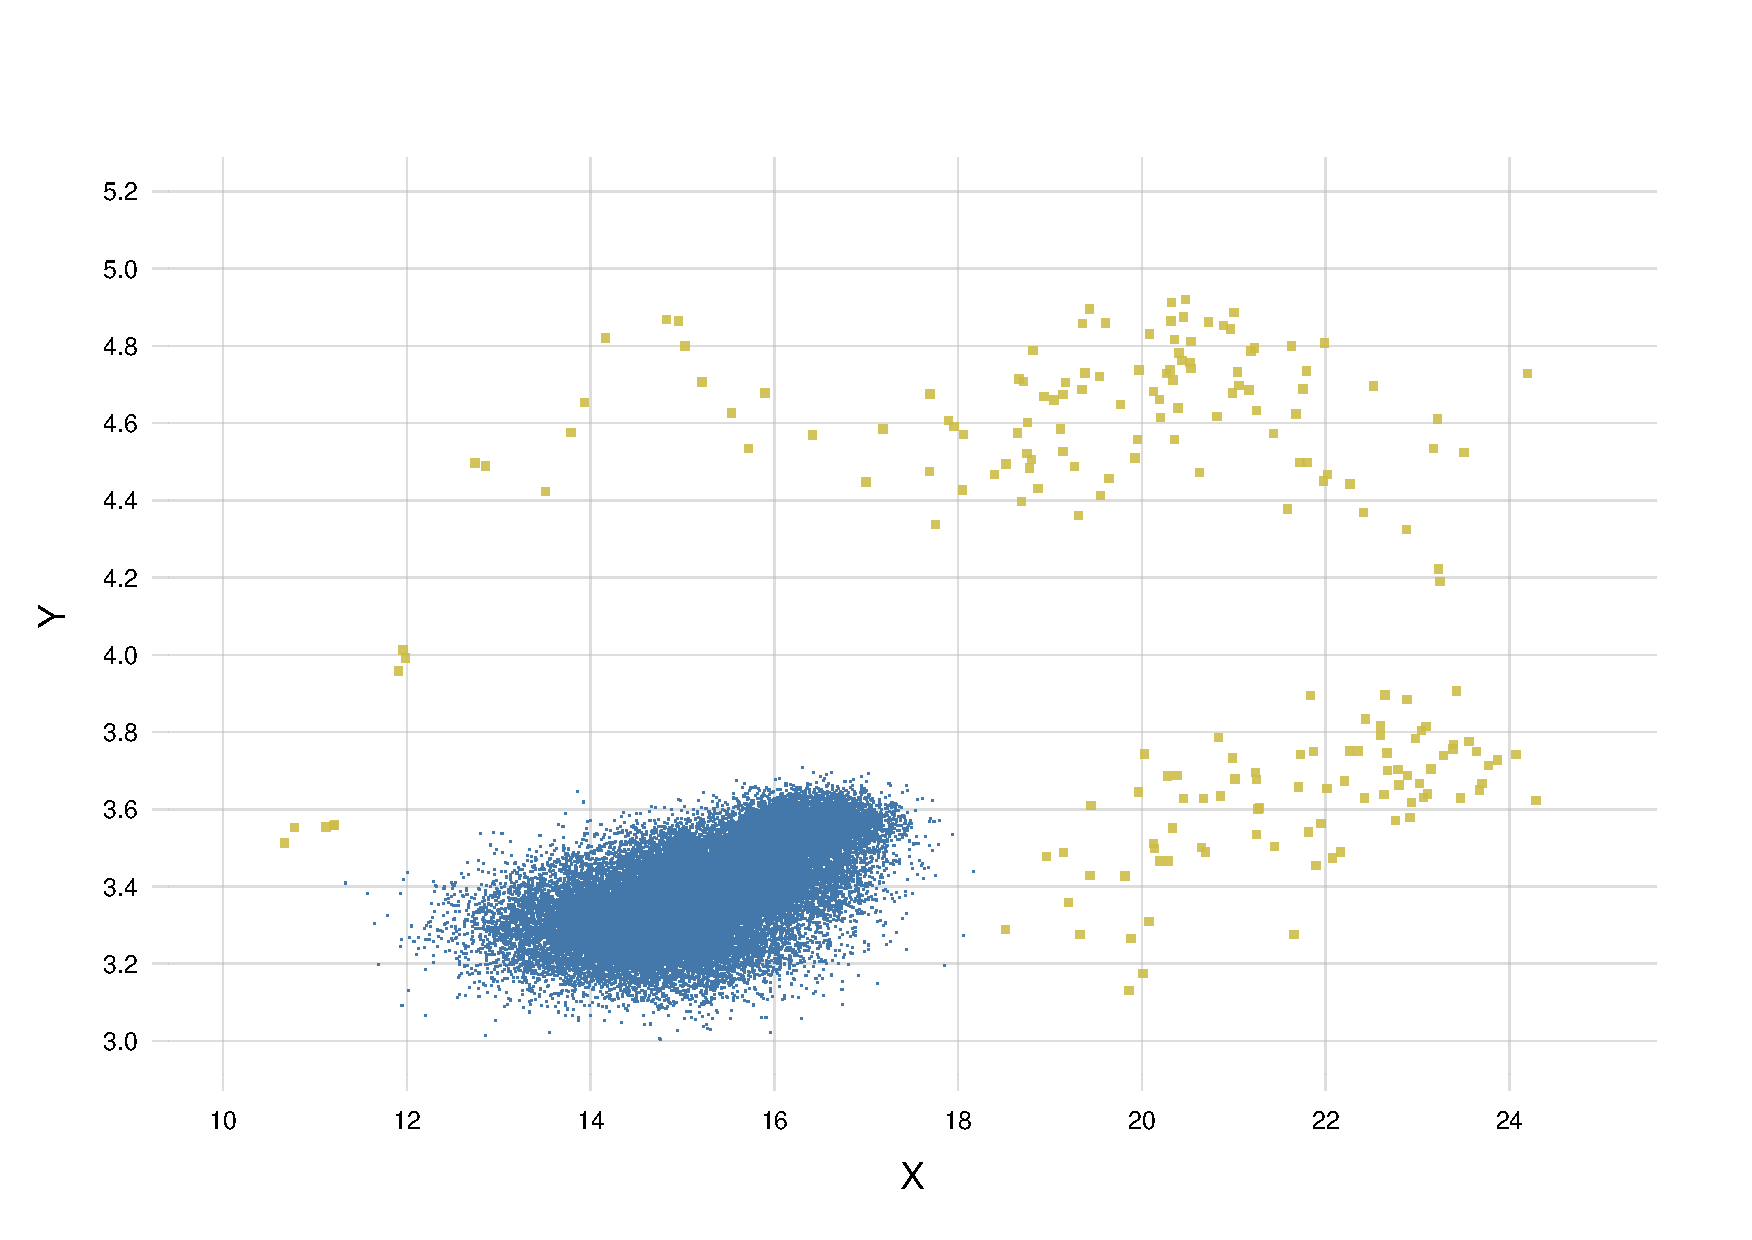
\includegraphics[width=0.49\linewidth]{exampledistr_unlikely_all.pdf}
  \hfill
  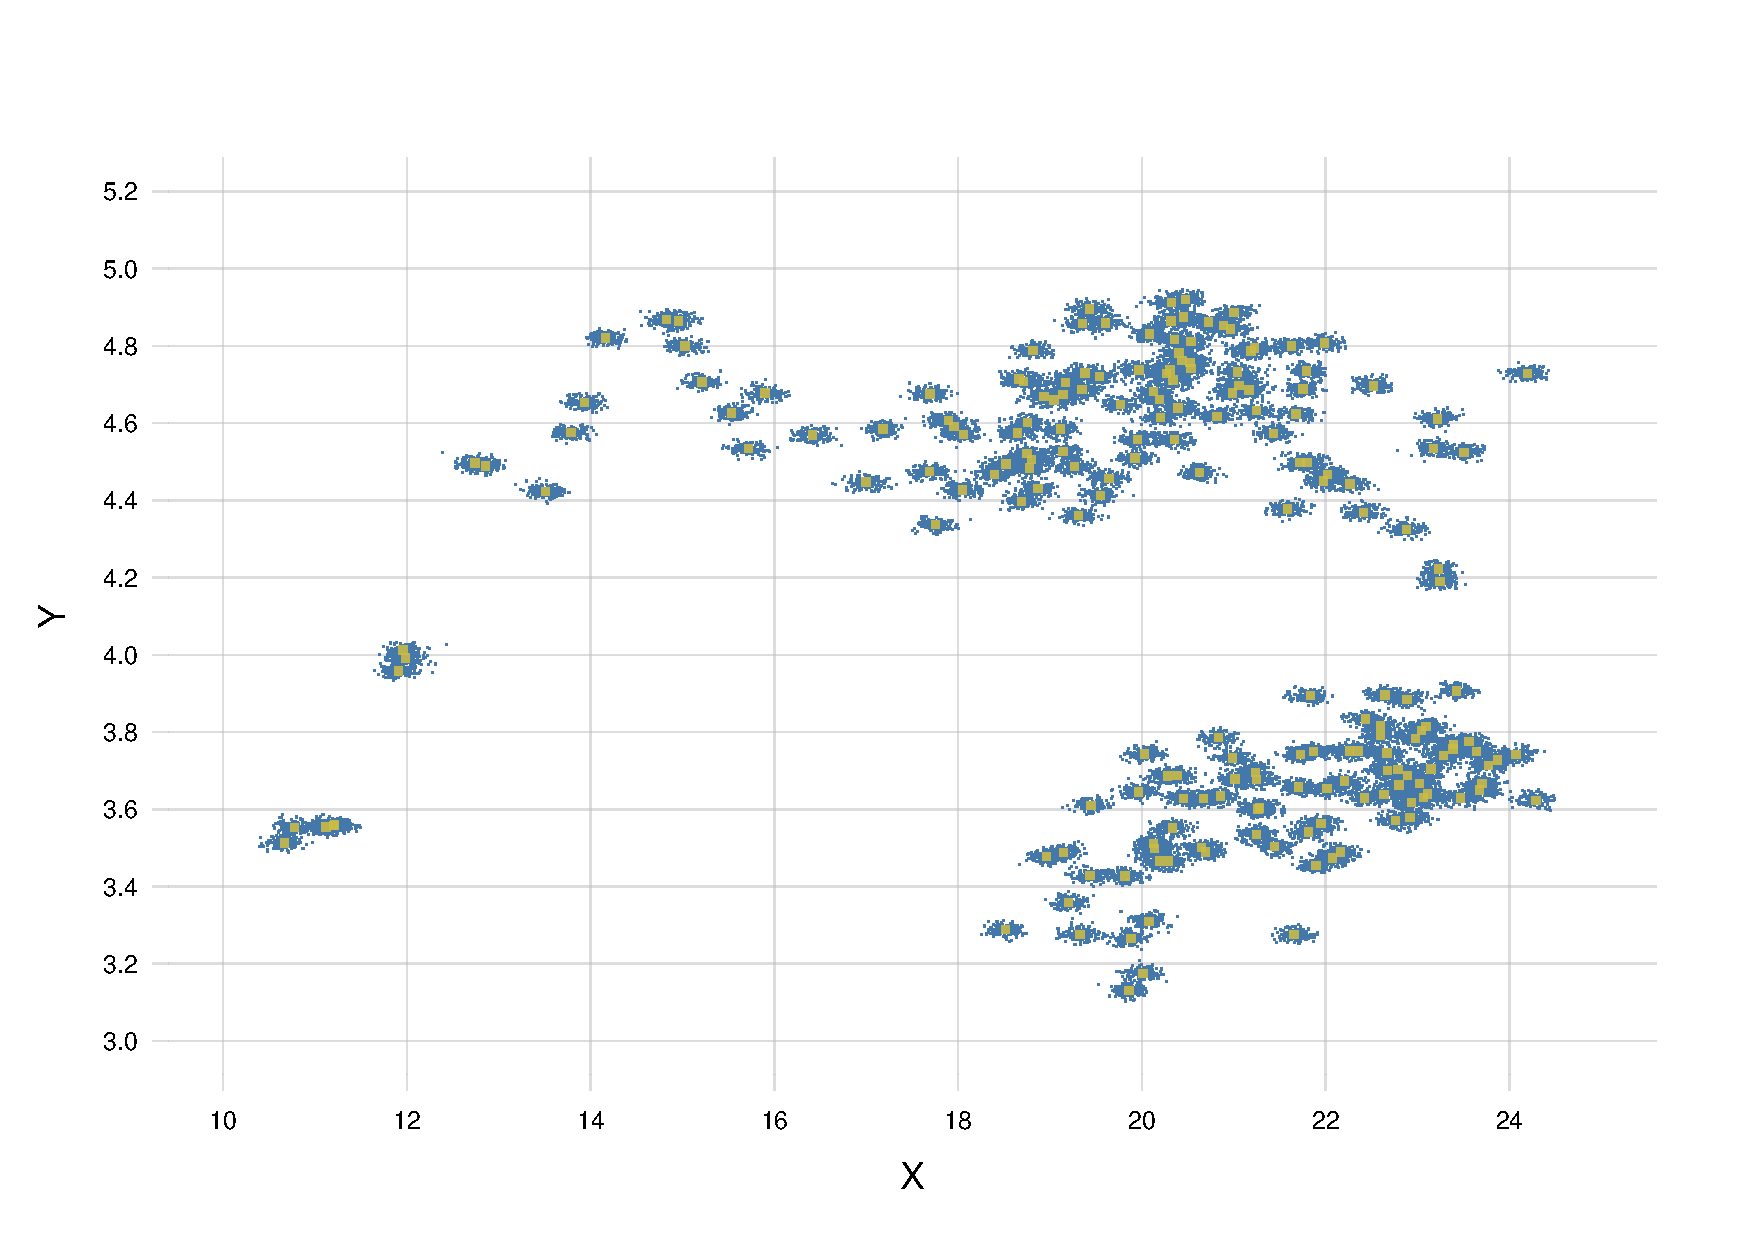
\includegraphics[width=0.49\linewidth]{exampledistr_strange_all.pdf}
  \caption{\mynotep{Upper-left: Sample data.
      Upper-right: candidate frequency distribution that fits the data and does not look unnatural.
      Lower-left: candidate distribution that might look natural but doesn't fit the sample data.
      Lower-right: candidate distribution that fits the data very well but looks unnatural.}}\label{fig:inferring_distribution}
\end{figure}%

\mynotep{Some more intuition and details about the maths, principles, and characteristics} \citep{dunsonetal2011,rossi2014,rasmussen1999}.

The \tjm\ computes the probabilities of all possible frequency distributions for the full population, and from these the joint probability distribution $\p(X,Y,Z,\dotsc)$ for all variates $X,Y,Z,\dotsc$ available in the dataset.

This is the\emph{ maximal amount of information} that can be extracted from the dataset. From it we can indeed quickly calculate any quantity typically outputted by specific or approximate algorithms. For example:
\begin{itemize}
\item \emph{Conditional probability, \enquote{discriminative} algorithms:} if we are interested in the probability of $Z$ given $X,Y$, we calculate $\p(Z \| X,Y) \defd \p(X,Y,Z)/\sum_{Z}\p(X,Y,Z)$.
\item \emph{Conditional probability, \enquote{generative} algorithms:} if we are interested in the probability of $X,Y$ given $Z$, we calculate $\p(X,Y\|Z) \defd \p(X,Y,Z)/\sum_{X,Y}\p(X,Y,Z)$.
\item \emph{Regression or classification:} if we are interested in the average value of $Z$ given $X,Y$, we calculate $\E(Z \| X,Y) \defd \sum_{Z}Z\,\p(Z\|X,Y)$. The \enquote{noise} around this average value is moreover given by $\p(Z-\E\|X,Y)$.
\item \emph{Functional regression:} if $Z$ turns out to be a function $f$ of $X,Y$, then the probability will be a delta distribution: $\p(Z\|X,Y) = \delt[Z-f(X,Y)]$.
  % We must remember that a function can always be represented by a probability distribution, but not vice versa.\footnote{The function $f\colon x \mapsto y=f(x)$ corresponds to the probability density $\p(y\|x) = \delt[y-f(x)]$, where $\delt$ is a delta distribution.}
  Thus, the \tjm\ always recovers a functional relationship if there is one, including its noise distribution.
\end{itemize}
We will see that no one of these quantities can be used \emph{alone} to solve our clinical decision problem for all future patients.

Use of the \tjm\ has further advantages and yields additional useful information:
\begin{itemize}
\item \emph{Discrete or continuous variates:} the variate to be prognosed can be not only binary or discrete, as in the present case, but also continuous.
\item \emph{Partially missing data:} data having missing values for some variates can be fully used, both in the learning dataset and in the prognostic results of new patients.
\item \emph{Maximal predictive power of the variates:} from the probability distribution $\p(X,Y,Z,\dotsc)$ we can calculate the mutual information between any two sets of variates, for example between $Z$ and $\set{X,Y}$. This quantity tells us what is the maximal predictive power -- which can be measured by accuracy or other metrics -- from one set to the other that can be achieved by any inference algorithm \citep{mackay1995_r2005,goodetal1968,coveretal1991_r2006}. Functional dependence is included as a special case; for example, a binary variate $Z$ is a function of $\set{X,Y}$ if and only if their mutual information \footnote{The \enquote{shannon} ($\mathrm{Sh}$) is a measurement unit of information, as specified by the \cite{iso2008c}.} equals $1\,\mathrm{Sh}$.
\item \emph{Variability owing to limited sample size:} we can calculate how much any of the quantities listed so far -- from average values to mutual information -- could change if more sample data were added to our dataset.
\end{itemize}

\medskip

For readers with an interest in machine learning and artificial intelligence, we briefly discuss the drawbacks of some popular inference algorithms with respect to the \tjm.

\emph{Neural networks and gaussian processes} are based on the assumption that there is a functional relationship from predictors to predictand,
possibly contaminated by a little noise, typically assumed gaussian. This is a very strong assumption, quite unrealistic for many kinds of variables considered in medicine. It can only be justified in the presence of informationally very rich predictors such as images. In our case the mutual information between predictors and the conversion variate is $0.14\,\mathrm{Sh}$, to be compared with $1\,\mathrm{Sh}$, if conversion were a function of the predictors, and with $0\,\mathrm{Sh}$, if conversion were completely unpredictable. See \sect~\mynotep{***} for further details. An additional deficiency of neural networks is that they do not yield any probabilities, even if there are many efforts to render such an output possible \citep{pearceetal2020,osbandetal2021,backetal2019}. Such an advance, however, would still not solve the final deficiency of neural networks and gaussian processes: they try to infer the predictand from the predictors but cannot be used for the reverse inference.

\emph{Random forests} also assume a functional relationship from predictors to predictand. This assumptions is mitigated when the predictand is a discrete variate; in this case a random forest can output an agreement score from its constituent decision trees. This score can give an idea of the underlying uncertainty, but it is not a probability,\footnote{It is sometimes called a \enquote{non-calibrated probability}, something akin to a \enquote{non-round circle}.} and therefore cannot be used in the decision-making stage, see \sect~\ref{sec:expected_utility_step}. It is possible to transform this score into a proper probability \citep{dyrlandetal2022b}, but this possibility does not solve the final deficiency of random forests: like neural networks, they try to infer the predictand from the predictors but cannot be used for the reverse inference.

\emph{Parametric models and machine-learning algorithms} such as logistic or linear regression, support-vector machines, or generalized linear models make even stronger assumptions than neural networks and random forests. They assume specific functional shapes or frequency distributions. Their use may be justified when we are extremely sure -- for instance thanks to underlying physical or biological knowledge -- of the validity of their assumptions; or when the computational resources are extremely scarce. But it is otherwise unnecessary to be hampered by their restrictive and often unrealistic assumptions.

\mynotew{Add note on \enquote{ensembling}: it does not give probabilities \citep[\sect~18.2]{murphy2022}}

\medskip

An important common deficiency of most inference algorithms mentioned above is that their inference only goes from predictors to predictands. In the next section we shall see that this limitation precludes -- or makes much riskier -- the prognostic use of the learning dataset for patients, such as Ariel, who belong to different populations.


\subsection{Application to the case study}
\label{sec:learn_application}

In our case study, the \tjm\ yields the following probabilities of main importance for the  application in the next sections:
  
\begin{table}[!h]
  \centering
  \begin{tabular}{lcccc}
    \hline\\[-1.5\jot]
    &{\small Olivia} &{\small Ariel} &{\small Bianca} &{\small Curtis}
    \\[\jot]
    {\small $\p(\text{conversion to AD} \| \text{predictors})$}&
    0.302&0.302&0.302&0.703
    \\
    {\small $\p(\text{predictors} \| \text{conversion to AD})/10^{-12}$}&
    8.97&8.97&8.97&1.14
    \\
    {\small $\p(\text{predictors} \| \text{no conversion to AD})/10^{-12}$}&
    18.6&18.6&18.6&0.343
    \\[\jot]
    \hline
  \end{tabular}
    \caption{\mynotew{Probabilities computed by the \tjm}}\label{tab:prob_likelihoods_patients}
\end{table}

As an illustration of the additional information provided by the \tjm, \fig~\ref{fig:freq_distribution_patients} shows the probability distributions for the full-population frequency of conversion to \ad\ for patients with predictor values equal to those of Olivia, Ariel, Bianca (left), and to those of Curtis (right). The probability $\p(\text{conversion to AD} \| \text{predictors}, \text{dataset})$ is equal to the average of such a distribution, as required by probability theory \citep[\eg][\sects~4.2--4.3]{bernardoetal1994_r2000}. We emphasize that the distributions shown in the figure are \emph{not} the \enquote{error} on these probabilities. There is an error on the probabilities, caused by finite computational precision, but it affects at most the third significant digit of the reported probabilities (all relative numerical errors are below 0.8\%, Curtis's two likelihoods being an exception at 2\%).

\begin{figure}[!t]% with figure
  \centering%
  \begin{minipage}{0.49\linewidth}\centering
    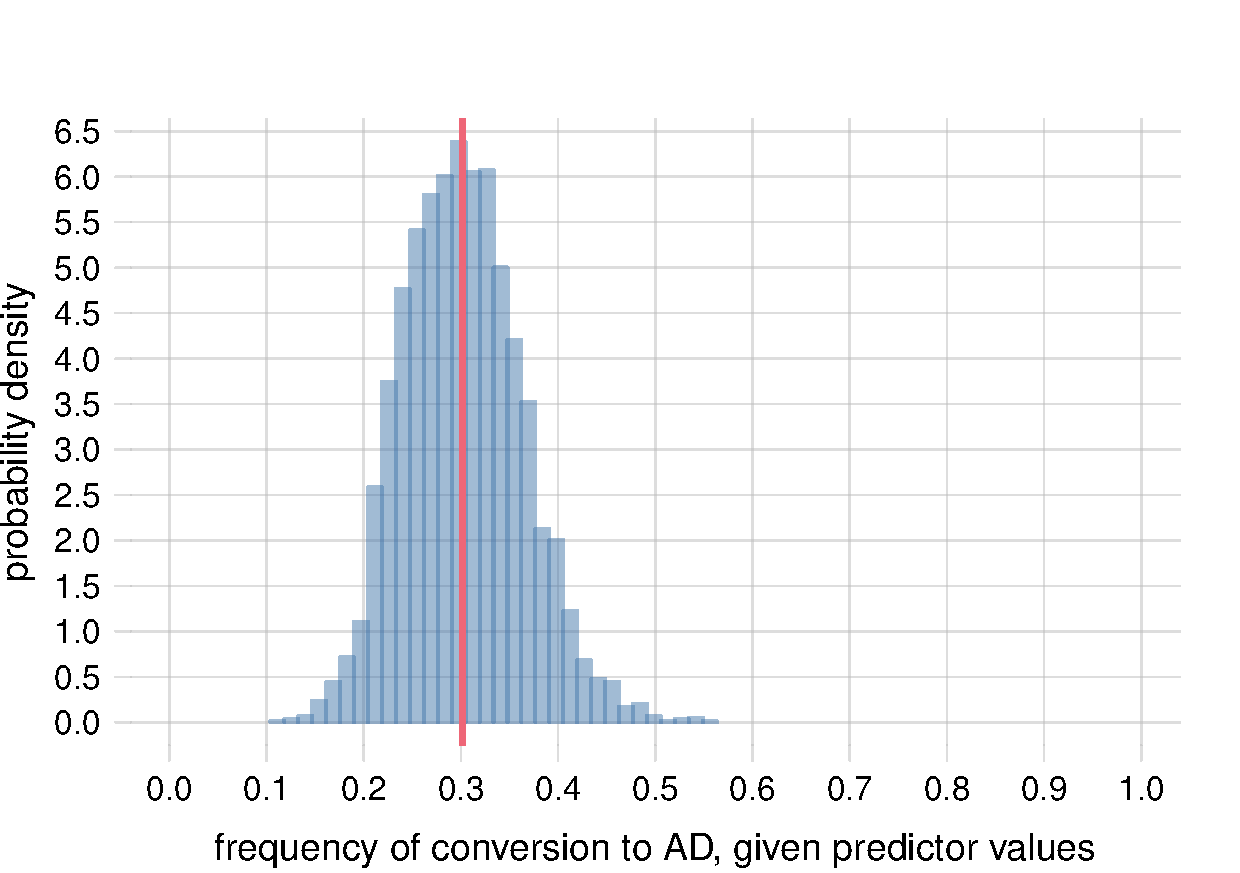
\includegraphics[width=\linewidth]{directprob_olivia.pdf}\\
    \footnotesize Olivia, Ariel, Bianca
  \end{minipage}
  \hfill
  \begin{minipage}{0.49\linewidth}\centering
    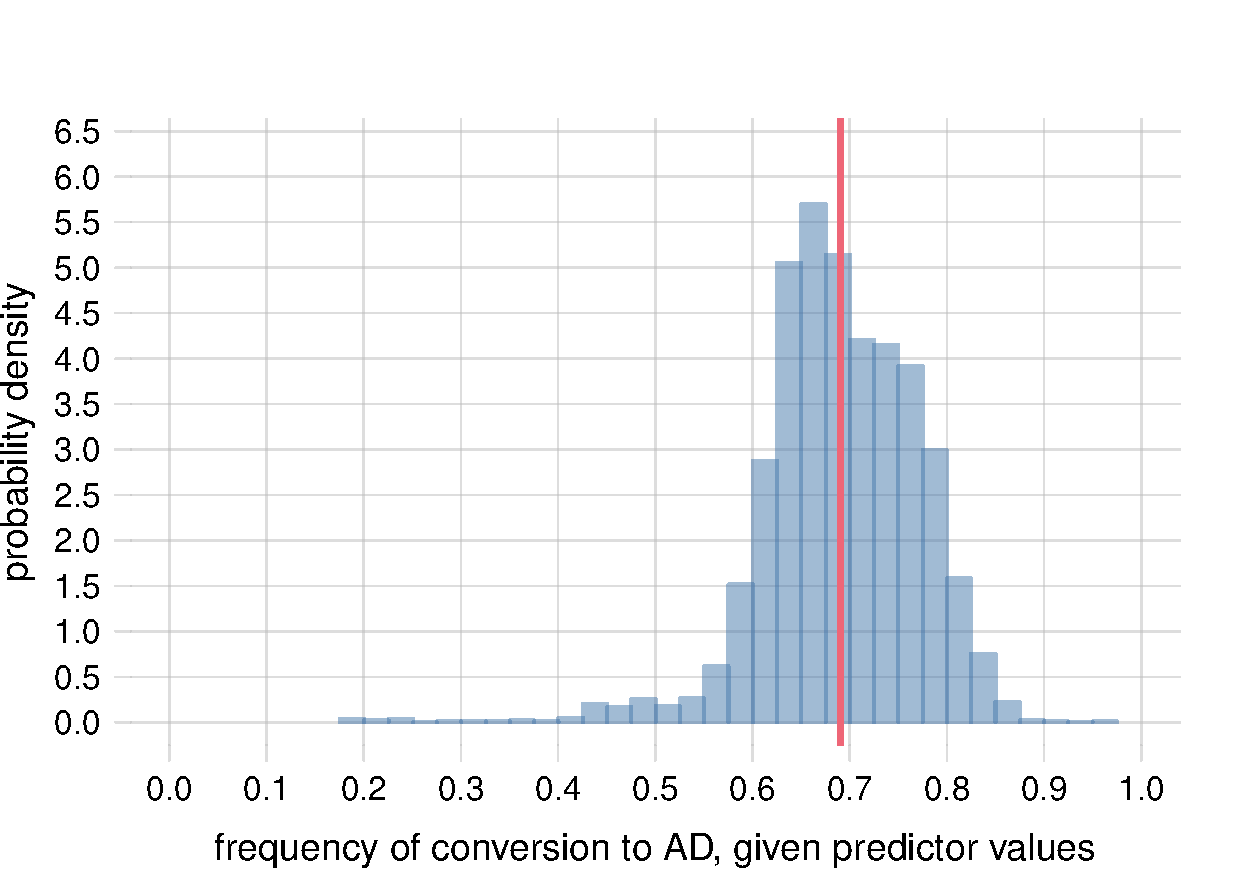
\includegraphics[width=\linewidth]{directprob_curtis.pdf}\\
    \footnotesize Curtis
  \end{minipage}
  \caption{Probability distributions for full-population frequency of conversion to AD, given Olivia, Ariel, Bianca's and Curtis's predictor. Red lines are the values of the probabilities  $\p(\text{conversion to AD} \| \text{predictors}, \text{dataset})$}\label{fig:freq_distribution_patients}
\end{figure}%



\medskip



%%%% MI given all minus ...
%      AVDEL30MIN_neuro RAVLT_immediate TRABSCOR_neuro AVDELTOT_neuro LRHHC_n_long
% mean            0.125           0.131          0.135          0.137        0.138
% sd              0.004           0.004          0.004          0.004        0.004
%      TRAASCOR_neuro CATANIMSC_neuro   AGE GDTOTAL_gds ANARTERR_neuro Gender_num_
% mean          0.139           0.139 0.139       0.140          0.140       0.140
% sd            0.004           0.004 0.004       0.004          0.004       0.004
%      Apoe4_   all
% mean  0.140 0.140
% sd    0.004 0.004


%%%% MI differences: 
%        all    Apoe4_ Gender_num_ ANARTERR_neuro GDTOTAL_gds      AGE CATANIMSC_neuro
% mean 0.000 0.0000121   0.0000939       0.000264    0.000295 0.000512        0.000561
% sd   0.009 0.0090000   0.0090000       0.009000    0.009000 0.009000        0.009000
%      TRAASCOR_neuro LRHHC_n_long AVDELTOT_neuro TRABSCOR_neuro RAVLT_immediate
% mean        0.00113      0.00187        0.00234        0.00438         0.00905
% sd          0.00900      0.00900        0.00900        0.00900         0.00800
%      AVDEL30MIN_neuro
% mean           0.0144
% sd             0.0080


\clearpage
\section{Population assessment and prior probability}
\label{sec:population_step}

\setlength{\intextsep}{0ex}% with wrapfigure
\setlength{\columnsep}{1ex}% with wrapfigure
\begin{wrapfigure}{r}{0.25\linewidth}% with wrapfigure
%\vspace{-1ex}%
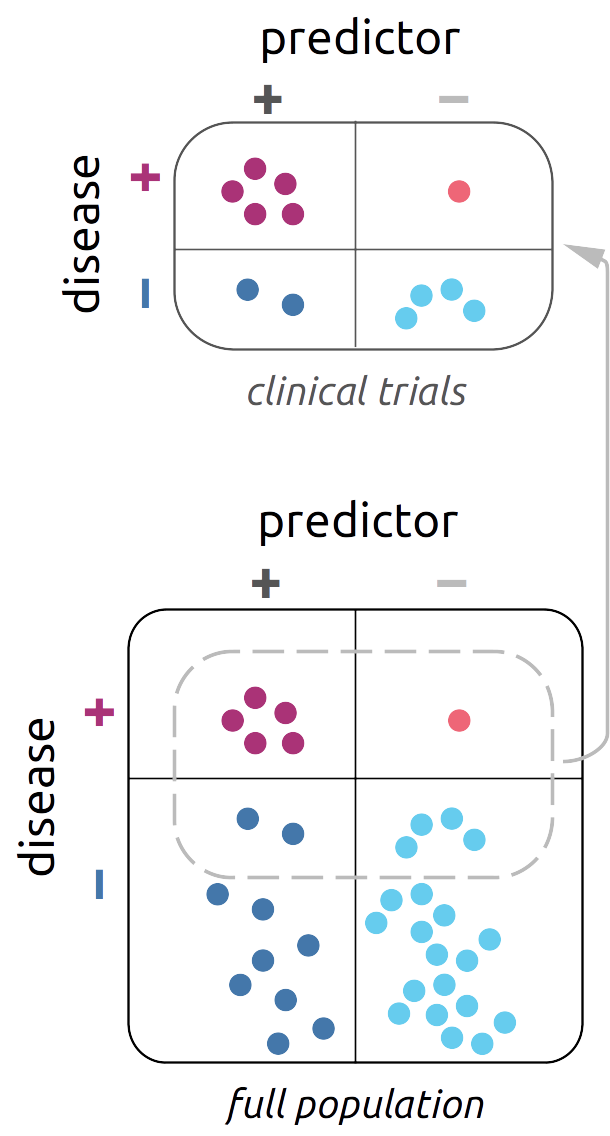
\includegraphics[width=\linewidth]{baseratefallacy3.png}%
% 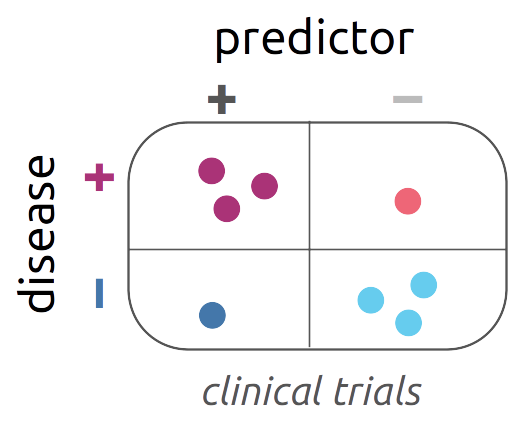
\includegraphics[width=\linewidth]{baseratetrials.png}\\[\jot]
% 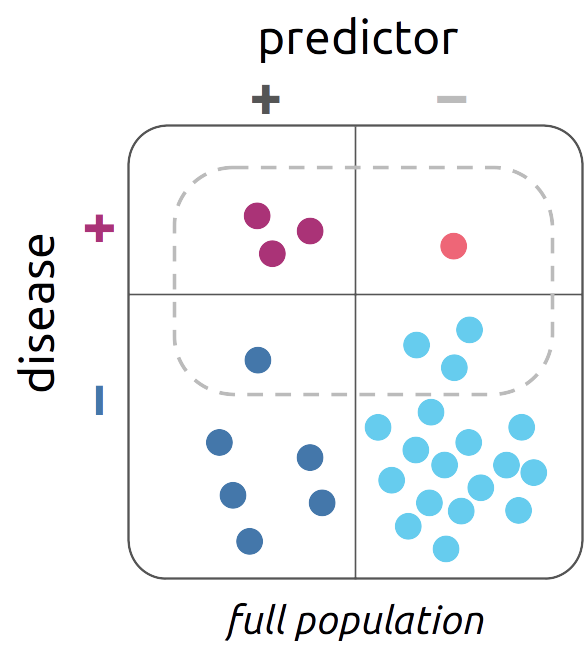
\includegraphics[width=\linewidth]{baseratepopulation.png}
\end{wrapfigure}%
Most medicine students learn about the \emph{base-rate fallacy} \citep{barhillel1980,jennyetal2018,sprengeretal2021,matthews1996}. Consider a large set of clinical trials, illustrated in the upper table on the side, where each dot represents, say, 10\,000 patients. In this sample dataset it is found that, among patients having a particular value \enquote{+} of some predictors (left column), 71.4\% (or 5/7, upper square) of them eventually developed a disease. The fallacy lies in judging that a new real patient from the full population, who has that particular predictor value, also has a 71.4\% probability of developing that disease. In fact, \emph{this probability will in general be different}. In our example it is 33.3\% (5/15), as can be seen in the lower table illustrating the full population. This difference would be noticed as soon as the inappropriate probability were used to make prognoses in the full population.

There is a discrepancy in the frequencies of predictand given predictors for the sample dataset and for the full population, because the proportion of positive vs negative disease cases in the latter has some value, 16.7\%/83.3\% in our example, whereas the samples for the trials (dashed line in the lower table) were chosen so as to have a 50\%/50\% proportion. This sampling procedure is called \enquote{class balancing} in machine learning \citep{provost2000,drummondetal2005,weissetal2003}. More generally this discrepancy can appear whenever a population and a sample dataset from it do not have the same frequency distribution for the predictand. In this case we cannot rely on the probabilities of \enquote{predictand given predictors} obtained from the sample dataset.

A little counting in the side figure reveals, however, that other frequencies may be relied upon. Consider the full population. Among all patients who developed the disease, 83.3\% (or 5/6, upper row) of them had the particular predictor value, while among those who did not develop the disease, 33.3\% (or 1/3, lower row) had the particular predictor value. \emph{And these frequencies are the same in the sample dataset}. These frequencies from the clinical trials can therefore be used to make a prognosis using Bayes's theorem:
\begin{equation}
  \label{eq:base-rate_correction}
  % \p(\textsf{\small predictand} \| \textsf{\small predictors}) \propto
  % \p(\textsf{\small predictors} \| \textsf{\small predictand},
  % \textsf{\small dataset})
  % \cdot   \p(\textsf{\small predictand} \| \textsf{\small population})
  \p(\textsf{\small predictand} \| \textsf{\small predictors}) =
  \frac{
    \p(\textsf{\small predictors} \| \textsf{\small predictand},
  \textsf{\small dataset})
  \cdot   \p(\textsf{\small predictand} \| \textsf{\small population})
}{\sum\limits_{\text{predictand}}
    \p(\textsf{\small predictors} \| \textsf{\small predictand},
  \textsf{\small dataset})
  \cdot   \p(\textsf{\small predictand} \| \textsf{\small population})
}
\end{equation}
In our example we find
\begin{equation}
  \label{eq:base-rate_correction_example}
 \begin{split}
  % \p(\textsf{\small predictand} \| \textsf{\small predictors}) \propto
  % \p(\textsf{\small predictors} \| \textsf{\small predictand},
  % \textsf{\small dataset})
  % \cdot   \p(\textsf{\small predictand} \| \textsf{\small population})
   \p(\textsf{\small disease+} \| \textsf{\small predictor+})
   &=
  \frac{
    \p(\textsf{\small predictor+} \| \textsf{\small disease+},
  \textsf{\small trials})
  \cdot   \p(\textsf{\small disease+} \| \textsf{\small population})
}{
  \biggl[\begin{aligned}
    &\p(\textsf{\small predictor+} \| \textsf{\small disease+},
  \textsf{\small trials}) 
  \cdot   \p(\textsf{\small disease+} \| \textsf{\small population})
  +{}\\[-0.5\jot]&\hspace{5em}
    \p(\textsf{\small predictor+} \| \textsf{\small disease\textminus},
  \textsf{\small trials})
  \cdot   \p(\textsf{\small disease\textminus} \| \textsf{\small population})
\end{aligned}\biggr]
} \\[2\jot]
&\approx
  \frac{ 0.833 \cdot 0.167}{0.833 \cdot 0.167 + 0.333 \cdot 0.833}
  = 0.33
  \end{split}
\end{equation}
which is indeed the correct full-population frequency.

If the samples of the clinical trials had been chosen with the same frequencies as the full population (no \enquote{class balancing}), then the probability $\p(\textsf{\small predictand} \| \textsf{\small predictors}, \textsf{\small dataset})$ from the dataset would be the appropriate one to use. But the probabilities $\p(\textsf{\small predictors} \| \textsf{\small predictand}, \textsf{\small dataset})$ together with Bayes's theorem as in \eqn~\eqref{eq:base-rate_correction} would also lead to exactly the same probability. We thus see that \emph{using the probabilities}
\[\p(\textsf{\small predictors} \| \textsf{\small predictand}, \textsf{\small dataset})\]
\emph{from the dataset is preferable to using} $\p(\textsf{\small predictand} \| \textsf{\small predictors}, \textsf{\small dataset})$. The former yield the same results as the latter when use of the latter is appropriate, and allow us to apply corrections when use of latter is inappropriate.

The superiority of using $\p(\textsf{\small predictors} \| \textsf{\small predictand}, \textsf{\small dataset})$ probabilities can be illustrated with a toy example. We split our learning dataset in two subsets:
\begin{itemize}
\item One with 361 datapoints and a ratio of 29.9\%/70.1\% of conversions to \ad\ vs stable \mci. This is used as learning set.
\item One with 343 datapoints and a ratio of 63.3\%/36.7\% of conversions to \ad\ vs stable \mci. This is used as a fictive full population.
\end{itemize}
No systematic sampling of any variates was made in this partition, besides the conversion variate.

We then make a prognosis for each of the 343 new patients with four approaches: (a) using the probabilities $\p(\textsf{\small predictand} \| \textsf{\small predictors}, \textsf{\small dataset})$, as typical of machine-learning algorithms; (b) using $\p(\textsf{\small predictors} \| \textsf{\small predictand}, \textsf{\small dataset})$ together with the base rate, as explained above; (c) tossing a coin; (d) always prognosing \enquote{conversion to \ad}, which guarantees 63.3\% correct prognoses owing to the base rate. Here is the accuracy (that is, the number of prognoses giving more than 50\% probability to the correct course) of each approach, ranked:

\medskip
  
\begin{table}[!h]
  \centering
  \begin{tabular}{cccc}
    \hline\\[-\jot]
    {\scriptsize predictand$\|$predictors}&{\scriptsize coin toss}&{\scriptsize always predict conversion}&{\scriptsize predictors$\|$predictand \amp\ base rate}
    \\[1\jot]
    37.3\% & 50\% & 63.3\% & 73.2\%\\[\jot]
    \hline
  \end{tabular}
\end{table}

\medskip
  
The \enquote{predictand$\|$predictors} approach leads to worse results than a coin toss because of its underlying base-rate fallacy. The \enquote{predictors$\|$predictand} approach instead leads to better results than simply always prognosing the most common base-rate outcome; this shows that the dataset can still provide useful statistical information despite its mismatched base rate. Inference algorithms that only yield \enquote{predictand$\|$predictors} outputs, unlike the \tjm, are incapable of extracting this useful information.

\medskip

The use of dataset probabilities different from $\p(\textsf{\small predictand} \| \textsf{\small predictors}, \textsf{\small dataset})$ can be necessary even when the dataset has statistics identical with the population it is sampled from. Typical cases are the prognosis of a patient that comes from a peculiar subpopulation or even from a different population. The first case happens for instance when the clinician has additional information not included among the predictor variates, such as the result of an additional clinical test, or family history. The second case happens for instance when the patient comes from a different geographical region. There is of course no sharp distinction between these two cases.

What is important is that in either case it can still be possible to use statistical information from the sample dataset to make prognoses. It is sufficient that some \emph{conditional} statistics may be applicable to the specific patient. For a patient coming from a different region, for example, it may be judged that the conditional probabilities $\p(\textsf{\small predictand} \| \textsf{\small predictors}, \textsf{\small dataset})$ still apply. In other words, the patient may still be considered of a member of the subpopulation having those specific predictor values.

This topic is complex and of extreme importance for inference, but its study is not the goal of the present work. We refer the readers to the brilliant paper by Lindley \amp\ Novick \citeyearpar{lindleyetal1981} for further discussion, and the works by \cite{malinasetal2004_r2016} and \cite{sprengeretal2021} about Simpson's paradox, to which this topic is related. \mynotez{Maybe add refs to Pearl (and Russell) about the notion of causality -- which is somewhat circular, however.}

Our main point here is that population variability and auxiliary clinical information are important factors that differentiate patients, and a personalized approach ought to take them into account. The method here presented does this naturally, allowing a great flexibility in selecting which statistical features of the sample dataset should be used for each new patient, and the integration of auxiliary clinical information in the form of a prior probability. As discussed in \sect~\ref{sec:learning_step}, the \tjm\ allows us to quickly calculate conditional probabilities $\p(Y\|X, \textsf{\small dataset})$ for any desired variate subsets $Y$ and $X$ required by the patient's relevant population.


% The situation discussed above generalizes and becomes more complicated as we consider multiple predictor and predictand variates. In general, of all probabilities $\p(\dotso\|\dotso)$ obtained from the dataset we should use those having in the conditional %(
% \enquote{$\|\dotso)$} any variate suspected to have dataset statistics different from those of the population of interest. The final desired probabilities are then obtained through Bayes's theorem, supplying additional corrected statistics.

% Let's clarify this with an example. In our dataset we observe a value $\textsf{GDS} = 1$ with a frequency of 32\% across all patients. Among the patients who later converted to \ad, the frequency is 36\%; whereas among those who remained with a stable \mci, the frequency is 28\%. Given a new patient, if we knew that 

\subsection{Application to the case study}
\label{sec:posterior_application}

In our present example, all statistics of the dataset are considered relevant for Olivia, Bianca, and Curtis. For these patients we can therefore use Bayes's theorem with the likelihoods of table~\ref{tab:prob_likelihoods_patients} and the dataset conversion rate of $0.463$ -- or equivalently directly the probabilities $\p(\textsf{\small conversion} \| \textsf{\small predictors}, \textsf{\small dataset})$ provided in the same table.

For Ariel, however, the clinician judges that a different base rate or prior probability of conversion should be used, equal to 65\%,  owing to her different geographical origin and family history. In her case we must use Bayes's theorem with the likelihoods of table~\ref{tab:prob_likelihoods_patients} and the prior probability of $0.65$.

The final probabilities of conversion to \ad\ for our four patients are reported in table~\ref{tab:posterior_patients}. Note how the final probability for Ariel is higher than that for Olivia and Bianca, even if the predictor data are the same for these three patients.

\medskip
\begin{table}[!h]
  \centering
  \begin{tabular}{lcccc}
    \hline\\[-1.5\jot]
    &{\small Olivia} &{\small Ariel} &{\small Bianca} &{\small Curtis}
    \\[\jot]
    {\small prior probability $\p(\text{conversion to AD} \| \text{aux info})$}&
    0.463&0.65&0.463&0.463
    \\
    {\small final probability $\p(\text{conversion to AD} \| \text{predictors}, \text{dataset}, \text{aux info})$}&
    0.302&0.47&0.302&0.703
    \\[\jot]
    \hline
  \end{tabular}
    \caption{Final probabilities of conversion computed from dataset and auxiliary information}\label{tab:posterior_patients}
\end{table}


% \subsection{Likelihood and posterior probability}
% \label{sec:posterior_step}

%  \citep{lindleyetal1981,sprengeretal2021,barhillel1980}


\section{Assessments of treatments and benefits, and final decision}
\label{sec:utilities_step}

A crucial point in clinical decision-making is this: the clinician needs to assess, not the presence (present or future) of a disease, but the \emph{risk} of its presence. Is there a difference? and why is it important?

In clinical practice we can rarely diagnose or prognose a medical condition with full certainty. Perfect classification is therefore impossible. But also a \enquote{most probable} classification, which may be enough in other contexts, is inadequate in clinical ones. The problem is that the clinician has to decide among different courses of actions, such as different treatments, more tests, and so on, and the optimal one depends on \emph{how probable} the medical condition is, not just on whether it is more probable than not.

Two examples illustrate this point. Say there is a dangerous treatment that extends the patient's lifetime by one year if the disease is actually on its course, but shortens the patient's lifetime by five years if the disease is actually not present. Obviously the clinician cannot prescribe the treatment just because the disease is \enquote{more probably present than not}. If 60 out of 100 treated similar patients actually develop the disease (so \enquote{more probable than not} is correct), the clinician has added $1 \times 60 = 60$ years \emph{but subtracted $\mathit{5 \times 40 = 240}$ years} from their combined lifespans. As an opposite example, say a less dangerous treatment extends the patient's lifespan by five years if the disease is on its course, but shortens it by one month if the disease is not present. In this case it may be advisable to undergo the treatment even if the disease is \emph{less} probably present than not. If 20 out of 100 treated similar patients develop the disease, the clinician has added $5 \times 20=100$ and subtracted $\tfrac{1}{12} \times 60=5$ years to their combined lifespans.

In both examples it is clearly important to assess the \emph{probability} that the patient will develop the disease. And our method, as explained in the previous sections, gives us such probabilities.

But the choice between treatments does not only rely on the probability of the medical condition. Here is where the differences between patients matter and vary the most. Consider again the second example above, about the less dangerous treatment. Let us add that the treatment would extend the lifespan by five years, but would also somewhat worsen the quality of life of the patient and the patient's family. Suppose our patient is quite old and tired, has had a happy life, and is now looking with a peaceful mind towards death as a natural part of life. Such a patient may prefer to forego the bother of the treatment and the additional five years even if the probability for the disease is quite high.

The benefits of the different treatments, and the probability thresholds at which one treatment becomes preferable to another, must therefore be judged primarily by the patient. Utility theory and maximization of expected utility allow clinician and patient to make such judgements and decisions in a coherent way \citetext{\citealp{soxetal1988_r2013,huninketal2001_r2014}; see also the clear and charming exposition by \citealp{lindley1971_r1988}}.

We summarize the main, patient-dependent procedure for decision making, and show how our computations so far fit perfectly with it.

The clinician first assesses and list the mutually exclusive courses of actions available for the specific patient. These could be treatments, more tests, do nothing, and so on. Often there are \emph{sequences} of decision available, but the utility framework can be applied to them as well \citetext{see references above and \citealp{raiffa1968_r1970}}. The list of courses of action is already patient-dependent: some alternatives may not be suitable (say, owing to allergies), some may be economically too costly, and so on.

Each course of action will have different consequences, which additionally depend on the patient's unknown clinical condition of interest. A treatment may have some consequences if the patient has or will develop the disease, and different consequences otherwise. The patient quantifies, with the clinician's guidance, the benefits and costs -- technically called \enquote{utilities} -- of such possible consequences. The quantification of utilities is not within the scope of the present work. The references cited above offer several guidelines and rules for numerically translating factors such as quality of life and expected lifespan into utilities.

The courses of actions, uncertain clinical conditions, and the quantified utilities $U$ of their consequences can be organized into a table of this form:
  \begin{center}
    \begin{tabular}{cccc}
      &{\small clinical condition $a$}&{\small clinical condition $b$}&{\small \ldots}
      \\[2\jot]
      {\small action $\alpha$} & $U_{\alpha a}$ & $U_{\alpha b}$ &$\dotso$ \\[\jot]
      {\small action $\beta$} & $U_{\beta a}$ & $U_{\beta b}$ &$\dotso$ \\[\jot]
      {\small \ldots} &$\dotso$&$\dotso$&$\dotso$
    \end{tabular}
  \end{center}
which can be compactly represented by a so-called \emph{utility matrix} $\bigl(U_{ij})$, the row index $i$ enumerating the actions, and the column index $j$ the clinical conditions. Note that the number of possible treatments and of clinical conditions do not need to be equal; generally they are not.

The \emph{expected utility} $\eU_{i}$ of an action $i$ is calculated as the expectation of its utilities $U_{ia}, U_{ib}, \dotsc$ with respect to the probabilities $\p(a), \p(b), \dotsc$ of the clinical conditions $a,b,\dotsc$:
\begin{equation}
  \label{eq:def_expected_utility}
  \eU_{i} \defd U_{ia}\, \p(a) + U_{ib}\, \p(b) + \dotsb
\end{equation}
Note that this corresponds to a matrix multiplication between the matrix of utilities and the vector of probabilities.

Finally, the recommended action is the one having \emph{maximal expected utility}.

\mynotep{Add a couple of comments about the inevitability of the rules of decision theory \citep{lindley1971_r1988}}

\subsection{Application to the case study}
\label{sec:expected_utility_application}

At present there are no treatments for \ad, nor preventive treatments \mynotew{true?}. But for the sake of our case study let us imagine that there are three mutually exclusive treatment options for prevention or retardation of the disease; call them $\beta$, $\gamma$, $\delta$. And denote the simple option of \enquote{no treatment} by $\alpha$. The clinical conditions to be considered are just two: the patient will have stable \mci, or will convert to \ad. Denote them by $\nAD$ and $\AD$.

We have therefore $4 \times 2 = 8$ possible consequences of the four treatments depending on the two clinical conditions. Our four patients and clinician quantify the utilities, arriving at the utility matrices shown in table~\ref{tab:utilities_patients}. Note that Olivia, Ariel, Curtis quantify the benefits of the treatments in exactly the same way, but Bianca's quantification differs slightly \mynotew{add an example of why}.

\medskip
\begin{table}[!h]
  \centering
  \begin{tabular}{lccccccc}
    \hline\\[-1.5\jot]
    &{\small Olivia} &&{\small Ariel} &&{\small Bianca} &&{\small Curtis}
    \\[\jot]
    $\begin{matrix}&\\
      \text{treatment }\alpha\\ 
      \text{treatment }\beta\\ 
      \text{treatment }\gamma\\ 
      \text{treatment }\delta
    \end{matrix}$
    &
    $
    \begin{gathered}
      \begin{smallmatrix}
        \nAD&\AD
      \end{smallmatrix}\\[-\jot]
\begin{bmatrix}10&0\\9&3\\8&5\\0&10\end{bmatrix}
\end{gathered}
$
    &&
    $\begin{gathered}
      \begin{smallmatrix}
        \nAD&\AD
      \end{smallmatrix}\\[-\jot]
      \begin{bmatrix}10&0\\9&3\\8&5\\0&10\end{bmatrix}\end{gathered}$
    &&
    $\begin{gathered}
      \begin{smallmatrix}
        \nAD&\AD
      \end{smallmatrix}\\[-\jot]
      \begin{bmatrix}10&0\\8&3\\7&5\\0&10\end{bmatrix}\end{gathered}$
    &&
    $\begin{gathered}
      \begin{smallmatrix}
        \nAD&\AD
      \end{smallmatrix}\\[-\jot]
      \begin{bmatrix}10&0\\9&3\\8&5\\0&10\end{bmatrix}\end{gathered}$
    \\[6\jot]
    \hline
  \end{tabular}
  \caption{Utility matrices for the four patients}\label{tab:utilities_patients}
\end{table}

The probabilities for the two medical conditions are those found in the previous section, reported in table~\ref{tab:posterior_patients}. For brevity we denote just by $\p(\AD)$ the probability of conversion given a patient's predictor values, and by $\p(\nAD)\equiv 1- \p(\AD)$ the complementary probability of stable \mci, given the same predictor values. The expected utilities of each treatment for each patient can then be easily computed. For example, for Olivia the expected utility of treatment $\beta$ is
\begin{equation}
  \label{eq:utility_olivia_example}
  \eU_{\beta} = 9 \cdot (1-0.463) + 3 \cdot 0.463 = 7.19
\end{equation}
The results for all patients are reported in table~\ref{tab:exp_utilities_patients}, with the maximal expected utilities in \textbf{boldface}.

\medskip
\begin{table}[!h]
  \centering
  \begin{tabular}{lcccc}
    \hline\\[-1.5\jot]
    &{\small Olivia} &{\small Ariel} &{\small Bianca} &{\small Curtis}
    \\[\jot]
    $\begin{matrix}
      \text{treatment }\alpha\\ 
      \text{treatment }\beta\\ 
      \text{treatment }\gamma\\ 
      \text{treatment }\delta\\[\jot]
      \text{optimal}
    \end{matrix}$
    &
    $\begin{matrix}6.98\\\bm{7.19}\\7.09\\3.02\\[\jot]\beta\end{matrix}$
    &
    $\begin{matrix}5.27\\6.16\\\bm{6.58}\\4.73\\[\jot]\gamma\end{matrix}$
    &
    $\begin{matrix}\bm{6.98}\\6.49\\6.40\\3.02\\[\jot]\alpha\end{matrix}$
    &
    $\begin{matrix}2.97\\4.78\\5.89\\\bm{7.03}\\[\jot]\delta\end{matrix}$
    \\[5\jot]
    \hline
  \end{tabular}
  \caption{Expected utilities and optimal treatment for our four patients}\label{tab:exp_utilities_patients}
\end{table}

% ##     olivia    ariel   curtis
% ## 1 0.698321 0.527060 0.297440
% ## 2 0.718993 0.616236 0.478464
% ## 3 0.709496 0.658118 0.589232
% ## 4 0.301679 0.472940 0.702560

% ##     bianca
% ## 1 0.698321
% ## 2 0.649161
% ## 3 0.639664
% ## 4 0.301679

 
% \subsection{Maximization of expected benefit}
% \label{sec:expected_utility_step}

%% Mutual-info results
% MI: 
%                               mean     sd
% GDTOTAL_gds               0.00052096 0.0003
% Gender_num_               0.00320230 0.0008
% Apoe4_                    0.00349680 0.0010
% AGE                       0.00616330 0.0010
% ANARTERR_neuro            0.00686160 0.0010
% TRAASCOR_neuro            0.01329100 0.0020
% TRABSCOR_neuro            0.02385100 0.0020
% CATANIMSC_neuro           0.02425800 0.0020
% LRHHC_n_long              0.02813100 0.0020
% noncog+demog              0.03598000 0.0030
% AVDELTOT_neuro            0.06025100 0.0030
% RAVLT_immediate           0.09243000 0.0040
% AVDEL30MIN_neuro          0.09397900 0.0040
% allminus_AVDEL30MIN_neuro 0.12548000 0.0040
% allminus_RAVLT_immediate  0.13083000 0.0040
% allminus_TRABSCOR_neuro   0.13546000 0.0040
% allminus_AVDELTOT_neuro   0.13761000 0.0040
% allminus_LRHHC_n_long     0.13797000 0.0040
% cog+demo                  0.13798000 0.0040
% allminus_TRAASCOR_neuro   0.13870000 0.0040
% allminus_CATANIMSC_neuro  0.13928000 0.0040
% allminus_AGE              0.13933000 0.0040
% allminus_GDTOTAL_gds      0.13956000 0.0040
% allminus_ANARTERR_neuro   0.13957000 0.0040
% allminus_Gender_num_      0.13974000 0.0040
% allminus_Apoe4_           0.13983000 0.0040
% all                       0.13984000 0.0040



\newpage
\section{Additional results provided by the \tjm}
\label{sec:additional_results}

The rich output of the \tjm\ allows us to make not only a fully personalized prognosis and clinical decision-making, but also many kinds of sensitivity checks.

It can be useful to know, for example, how important some predictors are for the prognosis. If the values of some predictors are unavailable for a patient, the clinician may thus decide whether it is preferable to acquire them, of whether they can be simply neglected. More generally, predictors that are too invasive or too expensive to obtain and do not make a real difference in the prognosis could be dropped altogether.

The \tjm\ allows us to compute the expected \enquote{predictive power}, for the full population of patients, of any set of predictors available in the dataset; and for any metric measuring this power, such as accuracy. A fact of paramount advantage is that \emph{the predictive power of a set of predictors found with the \tjm\ is the maximal one obtainable by \textbf{any} inference algorithm}; in other words it is an intrinsic property of that set of predictors. Thus, if the \tjm\ says that the accuracy obtainable with a given set of predictors is 70\%, then we know that no other inference algorithm of any kind can reach a higher accuracy than 70\%; and inference algorithms than reach lower accuracy can in principle be improved upon.

We show this kind of predictive-power computation for the present dataset. In our four-patient scenario it could be important for Curtis, whose value of Hippocampal Volume is missing (table~\ref{tab:patients_data}). His clinician thus wonders if its acquisition would lead to a much more informative prognosis.

We use two metrics of \enquote{predictive power} of a set of predictors: the mutual information~\citep{shannon1948,coveretal1991_r2006} between them and the event of conversion to \ad, and their accuracy. Mutual information is a model-free measure of the relation between two sets of variates; it has diverse operational interpretations \citep{mackay1995_r2005,woodward1953_r1964,minka1998d_r2003,goodetal1968,kelly1956,kullback1959_r1978} and international standards \citep{iso2008c}. A set of predictors and a binary variate (such as our conversion to \ad) have a mutual information of $1\,\mathrm{Sh}$ if and only if there is a deterministic function from the former to the latter.

We consider 15 sets of predictors:
\begin{itemize}
\item every predictor, used individually (12 sets);
\item all cognitive-test predictors used together, jointly with demographic information (Age and Sex);
\item APOE4, Hippocampal Volume, and demographic information, used together;
\item all predictors together minus one, excluding each single predictor in turn (12 sets);
\item all predictors jointly.
\end{itemize}

The expected mutual information and accuracy (on a 0--1 scale) for these sets are reported in \fig~\ref{fig:mutual_info}, ordered from bottom to top according to increasing mutual information. The ordering of mutual information and accuracy agree within the numerical computation error. The latter is reported as bars of $\pm$~one standard deviation.
\begin{figure}[!t]% with figure
  \centering%
  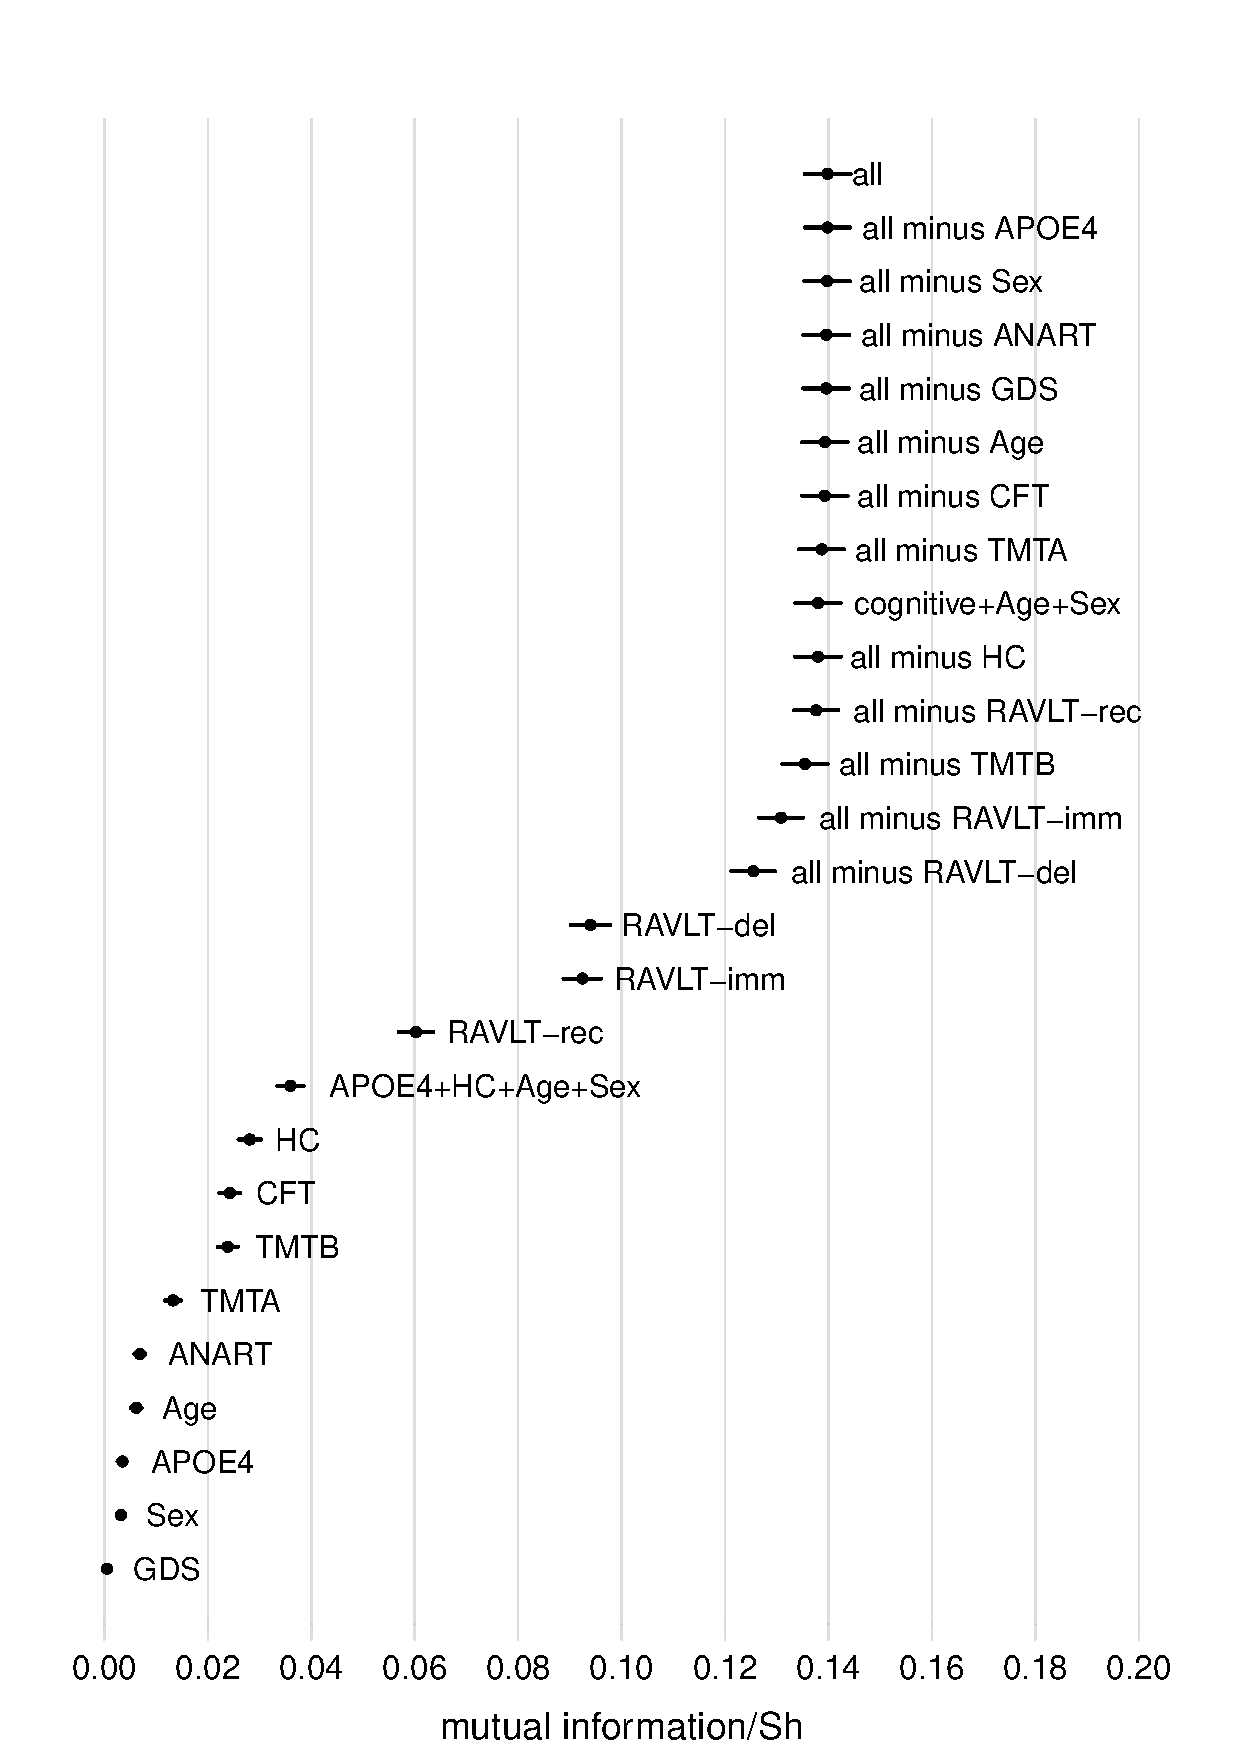
\includegraphics[width=0.494\linewidth]{plotMI.pdf}\hfill%
  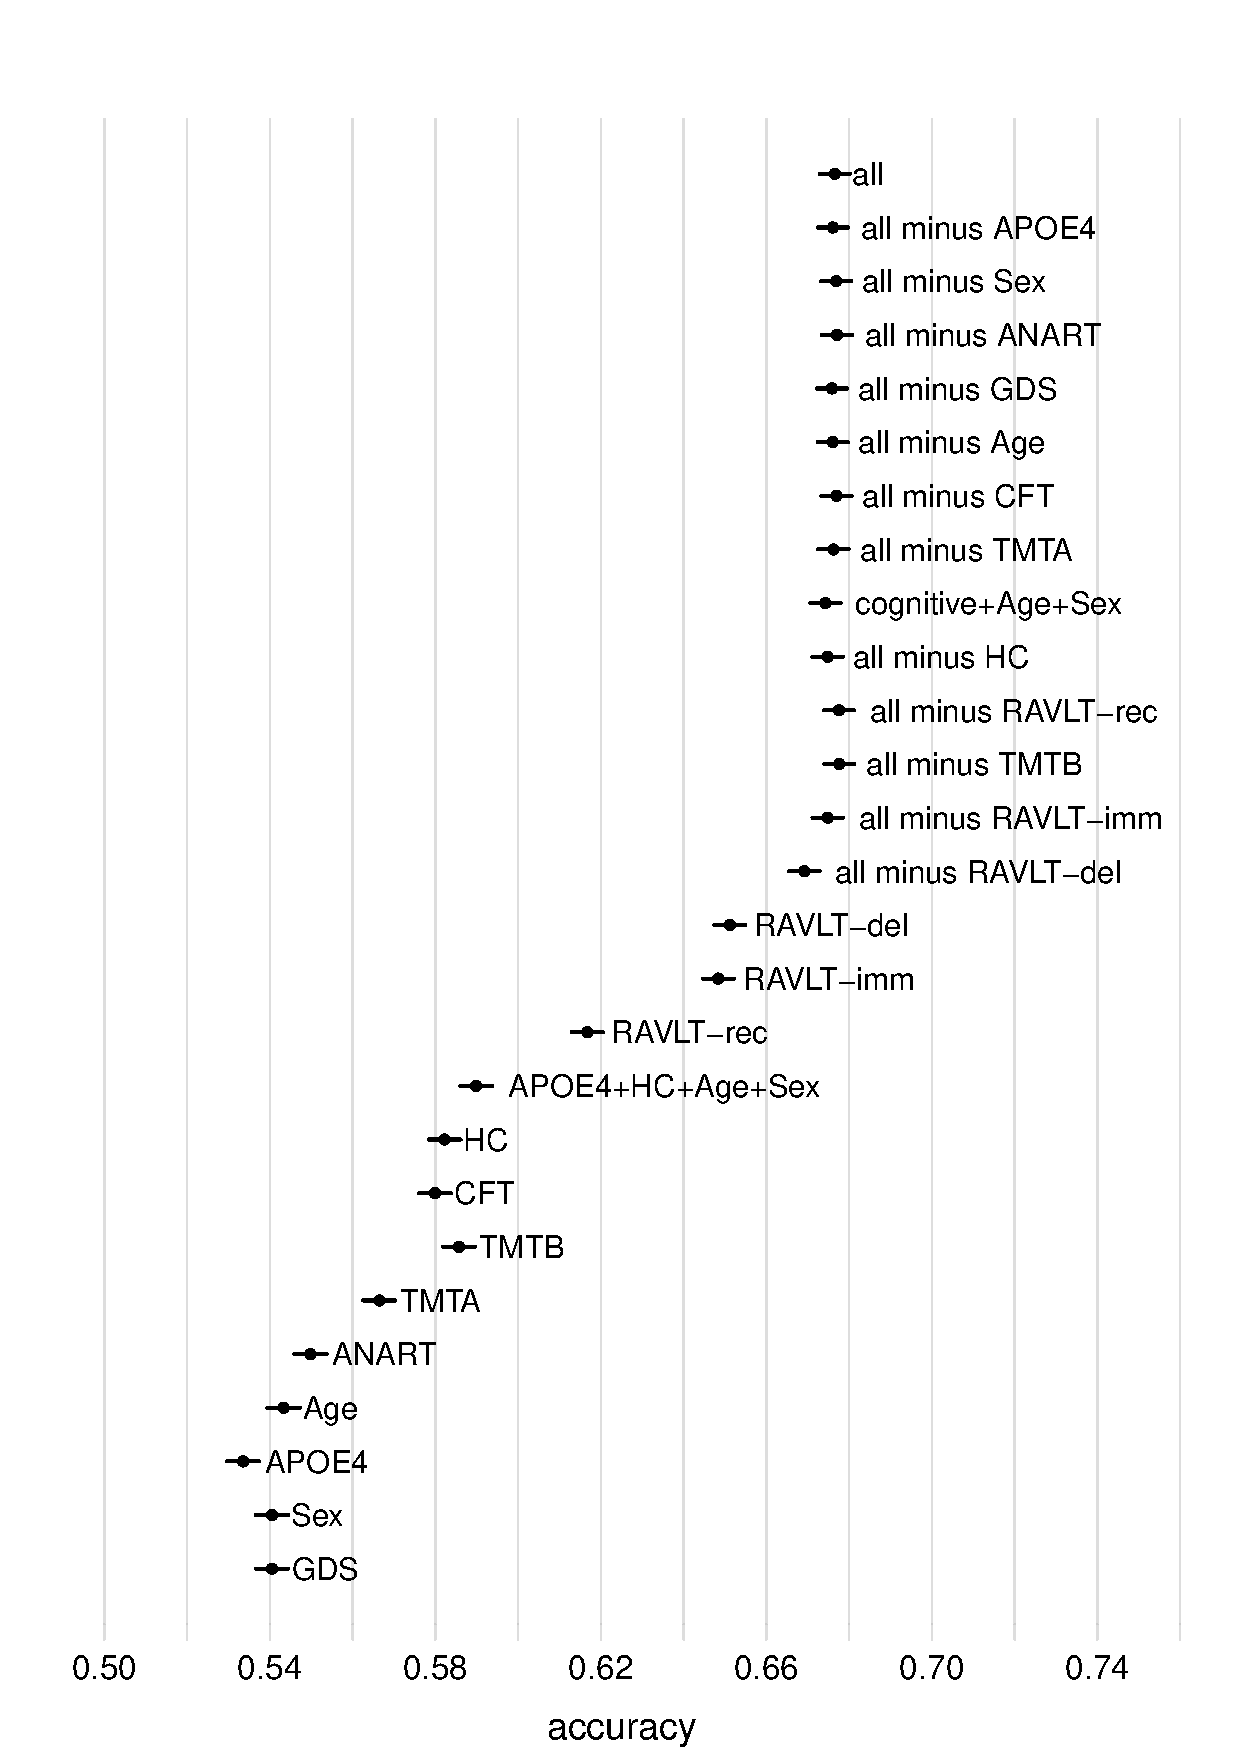
\includegraphics[width=0.494\linewidth]{plotAcc.pdf}%
  \caption{Mutual information and accuracy of several sets of predictors, for the prognosis of conversion to \ad. The bars show the numerical computation error ($\pm$~one standard deviation). Both graphs are ordered according to increasing mutual information (mutual-information and accuracy orderings agree within numerical error).}\label{fig:mutual_info}
\end{figure}%


The figure reveals several interesting findings, \emph{valid within the population selected for the dataset}, which can be compared with the analysis in  \cite[see especially Fig.~3 and Table~3]{ryeetal2022}:
\begin{itemize}
\item The set of 12 predictors considered in the present work \citep[and in ][]{ryeetal2022} can at most lead to a prognostic accuracy of around 68\%, for any inference algorithm. This fact agrees with the (completely independent) findings in \cite{ryeetal2022}, where a maximal accuracy of 68\% was found using an ensemble model; the present analysis also shows that that model managed to achieve the maximal accuracy possible with these predictors (but see \sect~\ref{sec:discussion} for limitations of that model.)
\item \textsf{APOE4}, \textsf{GDS}, \textsf{Age}, \textsf{Sex}, and to some degree \textsf{ANART} are poor predictors (within this population), when used alone and when used in combination with all other predictors. The latter point is evident from the fact that the mutual information of the combined predictors barely decrease if any one of these four predictors is omitted.
\item The combined cognitive and demographic variates are better predictors than the combined hippocampal, \textsf{APOE4}, and demographic variates.
\item \textsf{RAVLT-imm}, \textsf{RAVLT-del}, and to a lesser degree \textsf{RAVLT-rec} and Hippocampal Volume \citep[contrast this with]{ryeetal2022} are good predictors, both when used alone and when used in combination with all other predictors.
\end{itemize}

The \tjm\ shows that the omission of any one of the 12 predictors, except \textsf{RAVLT-del} and \textsf{RAVLT-imm}, does not lead to an appreciable decrease in mutual information (relative change of less than 3\%) or accuracy (relative decrease of 0.3\% or less). This puts the importance analysis of \citealp{ryeetal2022} into perspective. The exact quantification of these subtle differences is computationally quite expensive and we did not carry it out further.

It is important to keep in mind, however, that any ranking in \enquote{prognostic power} depends on the metric used. In a practical clinical application, the appropriate metric should be the patient's specific number of available treatments and their utility matrix \citep{dyrlandetal2022}. Use of the accuracy, as done above, assumes a patient with only two available treatments having utility matrix $\bigl[\begin{smallmatrix}1&0\\0&1\end{smallmatrix}\bigr]$.

\medskip

Regarding Curtis's missing value for Hippocampal Volume, his clinician can do this kind of sensitivity analysis using the output of the \tjm, calculating the probability distribution of Curtis's expected utilities (see table~\ref{tab:exp_utilities_patients}) \emph{if the Hippocampal Volume had been known}. The results of the 0.5\%--99.5\% intervals are as follows:

\medskip

\begin{table}[!h]
  \centering
  \begin{tabular}{rcc}
    \hline\\[-\jot]
    treatment&0.5\%&99.5\% \\[\jot]
    $\alpha$ & 2.97 & 2.99 \\
    $\beta$ & 4.78 & 4.79 \\
    $\gamma$ & 5.89 & 5.90 \\
    $\delta$ & \textbf{7.01} & \textbf{7.03}\\
    \hline
  \end{tabular}
\end{table}

(The four corresponding probability histograms, if plotted jointly, would look like vertical lines.)

It is clear that knowledge of this variate would not change the optimal treatment $\delta$. The clinician therefore proceeds without it.

% \begin{table}[!t]
%   \centering
%   \begin{tabular}{ll}
%     \hline\\[-1.5\jot]
%     {\small predictor set} &{\small mutual information/Sh}
%     \\[\jot]
% GDS               &0.0005  \\
% Sex               &0.0032  \\
% APOE4                    &0.0035  \\
% Age                       &0.006  \\
% ANART            &0.006  \\
% TMTA            &0.013  \\
% TMTB            &0.023  \\
% CFT           &0.024  \\
% HC              &0.028  \\
% \textbf{APOE4 + HC + demographic}         &0.036  \\
% RAVLT-rec            &0.060  \\
% RAVLT-imm           &0.092  \\
% RAVLT-del          &0.094  \\
% all minus RAVLT-del &0.125  \\
% all minus RAVLT-imm  &0.131  \\
% all minus TMTB   &0.135  \\
% \textbf{cognitive + demographic}            &0.138  \\
% all minus RAVLT-rec   &0.138  \\
% all minus HC     &0.138  \\
% all minus TMTA   &0.139  \\
% all minus CFT  &0.139  \\
% all minus Age              &0.139  \\
% all minus GDS      &0.140  \\
% all minus ANART   &0.140  \\
% all minus Sex      &0.140  \\
% all minus APOE4           &0.140  \\
% \textbf{all}                       &0.140  \\[\jot]
%     \hline 
%   \end{tabular}
%   \caption{Mutual information between various predictor sets and conversion to \ad. The mutual information is measured in shannons and has a maximum numerical error of $0.004\,\mathrm{Sh}$}\label{tab:mutual_info}
% \end{table}

\newpage
\section{Summary of the case study}
\label{sec:summary}


Summary in table~\ref{tab:summary}.

\begin{table}[!t]
  \centering
  \begin{tabular}{lcccc}
    &{\small Olivia} &{\small Ariel} &{\small Bianca} &{\small Curtis}
    \\[\jot]
    \hline\\[-1.5\jot]
    \emph{\small Predictor values}&&&& \\[\jot]
    Age&75.4&75.4&75.4&63.8 \\
    Sex&F&F&F&M \\
    HC${}/10^{-3}$&4.26&4.26&4.26&[missing] \\
    APOE4&N&N&N&Y \\
    ANART&18&18&18&15 \\
    CFT&21&21&21&14 \\
    GDS&3&3&3&2 \\
    RAVLT-im&36&36&36&20 \\
    RAVLT-del&5&5&5&0 \\
    RAVLT-rec&10&10&10&3 \\
    TMTA&21&21&21&36 \\
    TMTB&114&114&114&126
    \\[2\jot] \hline\\
    \emph{\small Outputs of \tjm}&&&& \\[\jot]
    {\small $\p(\AD \| \text{predictors})$}&
    0.302&0.302&0.302&0.703
    \\
    {\small $\p(\text{predictors} \| \AD)/10^{-12}$}&
    8.97&8.97&8.97&1.14
    \\
    {\small $\p(\text{predictors} \| \nAD)/10^{-12}$}&
    18.6&18.6&18.6&0.343
    \\[2\jot] \hline\\
    \emph{\small Additional information, final probability}&&&& \\[\jot]
    {\small auxiliary info}&
    {\small none}&
    {\small family history, base rate}&
    {\small none}&
    {\small none}\\
    {\small applicable dataset statistics}&
    {\small all}&
    {\small predictor$\|$predictand}&
    {\small all}&
    {\small all}\\
    {\small prior probability of conversion}&
    0.463&0.65&0.463&0.463
    \\[\jot]
    {\small final probability of conversion}&
    0.302&0.47&0.302&0.703
    \\[2\jot] \hline\\
    \emph{\small Available actions and utilities}&&&& \\[\jot]
    $
    \begin{matrix}
      &\begin{smallmatrix}\nAD&\AD\end{smallmatrix}\\
      \begin{smallmatrix}
      \text{treatment $\alpha$}\\
      \text{treatment $\beta$}\\
      \text{treatment $\gamma$}\\
      \text{treatment $\delta$}
    \end{smallmatrix}&
    \Biggl[\begin{smallmatrix}
      \hphantom{\nAD}&\hphantom{\AD}\\&\\&\\&
    \end{smallmatrix}\Biggr]
    \end{matrix}$
    &
    $\begin{bmatrix}10&0\\9&3\\8&5\\0&10\end{bmatrix}$
    &
    $\begin{bmatrix}10&0\\9&3\\8&5\\0&10\end{bmatrix}$
    &
    $\begin{bmatrix}10&0\\8&3\\7&5\\0&10\end{bmatrix}$
    &
    $\begin{bmatrix}10&0\\9&3\\8&5\\0&10\end{bmatrix}$
    \\[7\jot] \hline\\
    \emph{\small Expected utilities and optimal decision}&&&& \\[\jot]
    $\begin{matrix}
      \text{treatment }\alpha\\ 
      \text{treatment }\beta\\ 
      \text{treatment }\gamma\\ 
      \text{treatment }\delta\\[2\jot]
      \text{Optimal}
    \end{matrix}$
    &
    $\begin{matrix}6.98\\\bm{7.19}\\7.09\\3.02\\[2\jot]\bm{\beta}\end{matrix}$
    &
    $\begin{matrix}5.27\\6.16\\\bm{6.58}\\4.73\\[2\jot]\bm{\gamma}\end{matrix}$
    &
    $\begin{matrix}\bm{6.98}\\6.49\\6.40\\3.02\\[2\jot]\bm{\alpha}\end{matrix}$
    &
    $\begin{matrix}2.97\\4.78\\5.89\\\bm{7.03}\\[2\jot]\bm{\delta}\end{matrix}$
    \\[5\jot]
    \hline
  \end{tabular}
  \caption{\mynotew{Summary}}\label{tab:summary}
\end{table}



\newpage
\section{Discussion}
\label{sec:discussion}



\mynotez{Difficulty in assessing and quantifying additional info: Just ignoring it is not a solution and is unethical}

\mynotez{Subtly hidden disastrous consequences of not following normative decision theory: An algorithm can lead to saving 85\,000 patients out of 100\,000 and be deemed a success. But if the ideal algorithm had been used, 95\,000 patients would actually have been saved. What shall we say to the families of the 10\,000 patients who could have been saved but weren't?}

\subsection{Range of application of \tjm s}
\label{sec:rangeTJM}

The range of application of the \tjm\ used in the present study has two kinds of bound: computational and theoretical.

As mentioned in \sect~\ref{sec:learning_step} and explained in appendix~\ref{sec:maths_tjm}, the fact that the \tjm\ extracts all available information from the dataset also makes it computationally expensive. It is at present impossible to use with high-dimensional predictors (if our dataset had included a predictor such as a $128\times128\times128$ grayscale MRI image, the learning stage would have taken around 100 years). Approximate but much faster algorithms such as neural networks and random forests are thus, at present, still the only options with such predictors. There is, however, the interesting possibility of combining such fast algorithms together with a \tjm, as a post-processor of their raw output. This allows us to extract useful information usually hidden in such output at a low computational cost \citep{dyrlandetal2022b}. Such information can be then used for clinical decision making as illustrated in the present work.

As explained in \sect~\ref{sec:population_step}, the essentially sole assumption underlying the \tjm's inference and its practical used with new patients, is that the latter can be assumed to come, at least in some respects, from the same population as the learning dataset (in technical jargon, partial or conditional exchangeability applies). This precludes using the \tjm\ to forecast how the statistics of the full population could change in the future. However, the machine \emph{can} be used for time-dependent (transversal \mynotez{correct?}) inferences within a stable population, such as forecasts of the future time of disease onset, expected lifelength, and similar. For example, if data about the time of conversion to \ad\ were available in the dataset, the \tjm\ could forecast not only \emph{whether}, but also \emph{when} the conversion could take place.

\appendix
\renewcommand\thesection{\Alph{section}}
\section{Appendices}
\label{sec:appendices}

\subsection{Mathematical details about the \tjm}
\label{sec:maths_tjm}

% \setlength{\intextsep}{0ex}% with wrapfigure
% \setlength{\columnsep}{1ex}% with wrapfigure
% \begin{wrapfigure}{r}{0.25\linewidth}% with wrapfigure
% %\vspace{-1ex}%
% 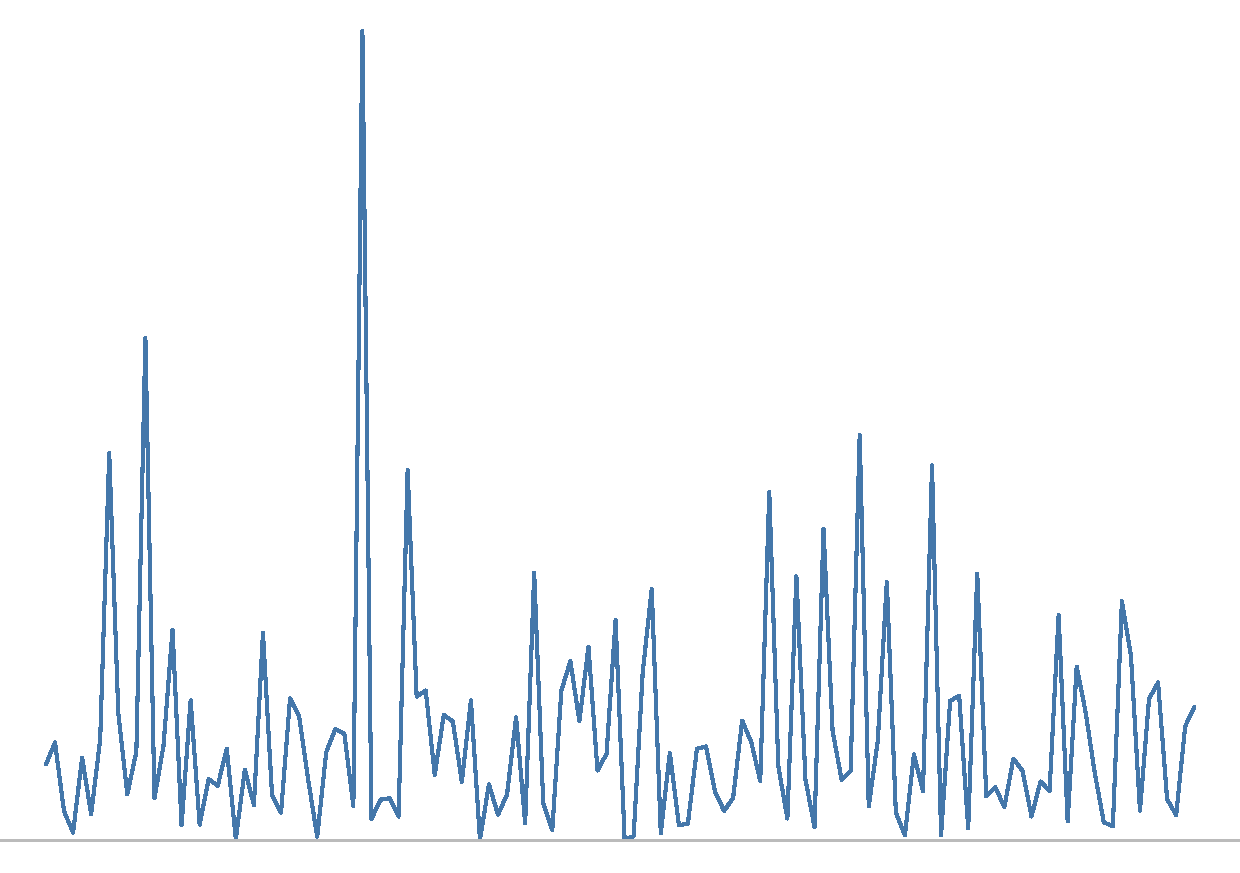
\includegraphics[width=\linewidth]{noisedistrnolines.pdf}%
% \end{wrapfigure}%
% The space of possible full-population frequency distributions has finite (owing to the finite precision of measurements) but very large number of dimensions. For our dataset it is around the order of $10^{20}$. Most distributions in such space, however, look like noise, as the example on the side, and are completely unrealistic as distributions for a \emph{full population}.

As discussed in \sect~\ref{sec:learning_step}, the \tjm\ explores the space of possible distributions of frequencies of all 13 variates listed in table~\ref{tab:patients_data}, for the full population of patients from which the dataset originates. In the present study it does so by using a total of 1535 independent parameters to represent the distributions, with roughly 190 parameters for each continuous or integer variate. As a crude intuition, it is as if we divided the range of each variate into 190 bins, and considered all possible frequency histograms over these. The actual parametrization is smarter, using parameters to represent less and less smooth traits of the distribution. We indeed expect the distribution for a full population to have some degree of smoothness, owing to physical and biological reasons. Actually, the number of parameters used is in principle infinite, because the machine gives a warning if the data indicates that more parameters are needed. In the present study the data indicates, on the contrary, that fewer than 250 parameters would be enough. More details on the mathematical representation can be found in \cite{dunsonetal2011}; see also \cite{rossi2014,rasmussen1999}.

\mynotep{Should I add a more precise description of the mathematical representation?}

\mynotep{Is the part below superfluous? I think it could be interesting for readers from machine learning}

There is a fundamental difference in how the \tjm\ and most popular machine-learning algorithms (including neural networks, random forests, support-vector machines, excluding gaussian processes) work. The latter do, at bottom, an optimization, looking for the minimum of some error function. The \tjm\ does a full \emph{space exploration} and \emph{averaging}, as explained in \sect~\ref{sec:learning_step}. Inference and generalization in fact essentially rely on averaging operations in problems such as the present one \citetext{de~Finetti's \citeyear{definetti1930} theorem; \citealp{definetti1937,dawid2013}; \citealp[\sects~4.2--4.3]{bernardoetal1994_r2000}; see also \citealp{selfetal1987}}. The optimization done by most machine-learning algorithms is an approximate form of averaging -- assuming or hoping that most of the mass to be averaged is around the extremum \citep[\chap~16]{mackay1992,murphy2012}. But the underlying necessity of a proper averaging becomes manifest in many of the obligatory procedures that go together with training a machine-learning algorithm; cross-validation for instance \citep{mackay1992b}. \mynotew{Add note: \enquote{ensembling} in ML is not this kind of averaging \citep[\sect~18.2]{murphy2022}}

This difference explains why the \tjm\ is computationally much more expensive than other algorithms, but also why its output is informationally so rich, and why it does not need any validation datasets, test datasets, other data splits, or cross-validation procedures \citetext{it can be proved that one of the internal computations of the machine is mathematically equivalent to doing $k$-fold cross-validations for \emph{all possible} data splits and $k$; see \eg\ \citealp{portamana2019b,fongetal2020}}.

\mynotew{one more remark about extremum-search being equivalent to making a choice, but the utilities are not controlled by the patient and not flexible.}



\mynotew{possibly add a plot showing the distributions considered reasonable by the machine}
\begin{figure}[!t]% with figure
  \centering%
  
\includegraphics[width=0.75\linewidth]{priorexamples_AVDEL30MIN_neuro.pdf}
  \caption{\mynotep{Examples of a-priori probable candidates of frequency distribution for a variate such as \textsf{RAVLT-del%AVDEL30MIN\_neuro
} or \textsf{RAVLT-rec%AVDELTOT\_neuro
}}}\label{fig:prior_distribution}
\end{figure}%









%%\setlength{\intextsep}{0ex}% with wrapfigure
%%\setlength{\columnsep}{0ex}% with wrapfigure
%\begin{figure}[p!]% with figure
%\begin{wrapfigure}{r}{0.4\linewidth} % with wrapfigure
%  \centering\includegraphics[trim={12ex 0 18ex 0},clip,width=\linewidth]{maxent_saddle.png}\\
%\caption{caption}\label{fig:comparison_a5}
%\end{figure}% exp_family_maxent.nb




\newpage
\hrule
\hrule



% {\color{yellow}\tiny For Original Research Articles \citep{conference}, Clinical Trial Articles \citep{article}, and Technology Reports \citep{patent}, the introduction should be succinct, with no subheadings \citep{book}. For Case Reports the Introduction should include symptoms at presentation \citep{chapter}, physical exams and lab results \citep{dataset}.

% }



% \section{Article types}

% For requirements for a specific article type please refer to the Article Types on any Frontiers journal page. Please also refer to  \href{http://home.frontiersin.org/about/author-guidelines#Sections}{Author Guidelines} for further information on how to organize your manuscript in the required sections or their equivalents for your field

% % For Original Research articles, please note that the Material and Methods section can be placed in any of the following ways: before Results, before Discussion or after Discussion.

% \section{Manuscript Formatting}

% \subsection{Heading Levels}

% %There are 5 heading levels

% \subsection{Level 2}
% \subsubsection{Level 3}
% \paragraph{Level 4}
% \subparagraph{Level 5}

% \subsection{Equations}
% Equations should be inserted in editable format from the equation editor.

% \begin{equation}
% \sum x+ y =Z\label{eq:01}
% \end{equation}

% \subsection{Figures}
% Frontiers requires figures to be submitted individually, in the same order as they are referred to in the manuscript. Figures will then be automatically embedded at the bottom of the submitted manuscript. Kindly ensure that each table and figure is mentioned in the text and in numerical order. Figures must be of sufficient resolution for publication \href{https://www.frontiersin.org/about/author-guidelines#ImageSizeRequirements}{see here for examples and minimum requirements}. Figures which are not according to the guidelines will cause substantial delay during the production process. Please see \href{https://www.frontiersin.org/about/author-guidelines#FigureRequirementsStyleGuidelines}{here} for full figure guidelines. Cite figures with subfigures as figure \ref{fig:Subfigure 1} and \ref{fig:Subfigure 2}.


% \subsubsection{Permission to Reuse and Copyright}
% Figures, tables, and images will be published under a Creative Commons CC-BY licence and permission must be obtained for use of copyrighted material from other sources (including re-published/adapted/modified/partial figures and images from the internet). It is the responsibility of the authors to acquire the licenses, to follow any citation instructions requested by third-party rights holders, and cover any supplementary charges.
% %%Figures, tables, and images will be published under a Creative Commons CC-BY licence and permission must be obtained for use of copyrighted material from other sources (including re-published/adapted/modified/partial figures and images from the internet). It is the responsibility of the authors to acquire the licenses, to follow any citation instructions requested by third-party rights holders, and cover any supplementary charges.

% \subsection{Tables}
% Tables should be inserted at the end of the manuscript. Please build your table directly in LaTeX.Tables provided as jpeg/tiff files will not be accepted. Please note that very large tables (covering several pages) cannot be included in the final PDF for reasons of space. These tables will be published as \href{http://home.frontiersin.org/about/author-guidelines#SupplementaryMaterial}{Supplementary Material} on the online article page at the time of acceptance. The author will be notified during the typesetting of the final article if this is the case. 

% \section{Nomenclature}

% \subsection{Resource Identification Initiative}
% To take part in the Resource Identification Initiative, please use the corresponding catalog number and RRID in your current manuscript. For more information about the project and for steps on how to search for an RRID, please click \href{http://www.frontiersin.org/files/pdf/letter_to_author.pdf}{here}.

% \subsection{Life Science Identifiers}
% Life Science Identifiers (LSIDs) for ZOOBANK registered names or nomenclatural acts should be listed in the manuscript before the keywords. For more information on LSIDs please see \href{https://www.frontiersin.org/about/author-guidelines#Nomenclature}{Inclusion of Zoological Nomenclature} section of the guidelines.


% \section{Additional Requirements}

% For additional requirements for specific article types and further information please refer to \href{http://www.frontiersin.org/about/AuthorGuidelines#AdditionalRequirements}{Author Guidelines}.

\section*{Conflict of Interest Statement}
%All financial, commercial or other relationships that might be perceived by the academic community as representing a potential conflict of interest must be disclosed. If no such relationship exists, authors will be asked to confirm the following statement: 

The authors declare that the research was conducted in the absence of any commercial or financial relationships that could be construed as a potential conflict of interest.

\section*{Author Contributions}

The authors were too immersed in the development of the present work to keep a detailed record of who did what.

% The Author Contributions section is mandatory for all articles, including articles by sole authors. If an appropriate statement is not provided on submission, a standard one will be inserted during the production process. The Author Contributions statement must describe the contributions of individual authors referred to by their initials and, in doing so, all authors agree to be accountable for the content of the work. Please see  \href{https://www.frontiersin.org/about/policies-and-publication-ethics#AuthorshipAuthorResponsibilities}{here} for full authorship criteria.

\section*{Funding}
Details of all funding sources should be provided, including grant numbers if applicable. Please ensure to add all necessary funding information, as after publication this is no longer possible.

\section*{Acknowledgments}
This is a short text to acknowledge the contributions of specific colleagues, institutions, or agencies that aided the efforts of the authors.

\section*{Supplemental Data}
 \href{http://home.frontiersin.org/about/author-guidelines#SupplementaryMaterial}{Supplementary Material} should be uploaded separately on submission, if there are Supplementary Figures, please include the caption in the same file as the figure. LaTeX Supplementary Material templates can be found in the Frontiers LaTeX folder.

\section*{Data Availability Statement}
The datasets [GENERATED/ANALYZED] for this study can be found in the [NAME OF REPOSITORY] [LINK].
% Please see the availability of data guidelines for more information, at https://www.frontiersin.org/about/author-guidelines#AvailabilityofData

\bibliographystyle{Frontiers-Harvard} %  Many Frontiers journals use the Harvard referencing system (Author-date), to find the style and resources for the journal you are submitting to: https://zendesk.frontiersin.org/hc/en-us/articles/360017860337-Frontiers-Reference-Styles-by-Journal. For Humanities and Social Sciences articles please include page numbers in the in-text citations 
%\bibliographystyle{Frontiers-Vancouver} % Many Frontiers journals use the numbered referencing system, to find the style and resources for the journal you are submitting to: https://zendesk.frontiersin.org/hc/en-us/articles/360017860337-Frontiers-Reference-Styles-by-Journal
\bibliography{portamanabib}

%%% Make sure to upload the bib file along with the tex file and PDF
%%% Please see the test.bib file for some examples of references

%% \section*{Figure captions}

%%% Please be aware that for original research articles we only permit a combined number of 15 figures and tables, one figure with multiple subfigures will count as only one figure.
%%% Use this if adding the figures directly in the mansucript, if so, please remember to also upload the files when submitting your article
%%% There is no need for adding the file termination, as long as you indicate where the file is saved. In the examples below the files (logo1.eps and logos.eps) are in the Frontiers LaTeX folder
%%% If using *.tif files convert them to .jpg or .png
%%%  NB logo1.eps is required in the path in order to correctly compile front page header %%%

% \begin{figure}[h!]
% \begin{center}
% 
\includegraphics[width=10cm]{logo1}% This is a *.eps file
% \end{center}
% \caption{ Enter the caption for your figure here.  Repeat as  necessary for each of your figures}\label{fig:1}
% \end{figure}

% \setcounter{figure}{2}
% \setcounter{subfigure}{0}
% \begin{subfigure}
% \setcounter{figure}{2}
% \setcounter{subfigure}{0}
%     \centering
%     \begin{minipage}[b]{0.5\textwidth}
%         
\includegraphics[width=\linewidth]{logo1.eps}
%         \caption{This is Subfigure 1.}
%         \label{fig:Subfigure 1}
%     \end{minipage}  
   
% \setcounter{figure}{2}
% \setcounter{subfigure}{1}
%     \begin{minipage}[b]{0.5\textwidth}
%         
\includegraphics[width=\linewidth]{logo2.eps}
%         \caption{This is Subfigure 2.}
%         \label{fig:Subfigure 2}
%     \end{minipage}

% \setcounter{figure}{2}
% \setcounter{subfigure}{-1}
%     \caption{Enter the caption for your subfigure here. \textbf{(A)} This is the caption for Subfigure 1. \textbf{(B)} This is the caption for Subfigure 2.}
%     \label{fig: subfigures}
% \end{subfigure}

%%% If you don't add the figures in the LaTeX files, please upload them when submitting the article.
%%% Frontiers will add the figures at the end of the provisional pdf automatically
%%% The use of LaTeX coding to draw Diagrams/Figures/Structures should be avoided. They should be external callouts including graphics.

\end{document}
